\documentclass[11pt,a4paper]{article}

% --- Packages ---
\usepackage[utf8]{inputenc}
\usepackage[T1]{fontenc}
\usepackage{amsmath,amssymb,amsfonts}
\usepackage{graphicx}
\usepackage{booktabs}
\usepackage{hyperref}
\usepackage[numbers,sort&compress]{natbib}
\usepackage[margin=1in]{geometry}
\usepackage{algorithm}
\usepackage{algorithmic}
\usepackage{multirow}
\usepackage{caption}
\usepackage{subcaption}
\usepackage{xcolor}
\usepackage{float}

% --- Hyperref setup ---
\hypersetup{
    colorlinks=true,
    linkcolor=blue,
    citecolor=blue,
    urlcolor=blue
}

% --- Custom commands ---
\newcommand{\R}{\mathbb{R}}
\newcommand{\E}{\mathbb{E}}
\newcommand{\Prob}{\mathbb{P}}

\title{Continuous Hidden Markov Models for Equity and Volatility Index Dynamics:\\Gaussian, Student-t, and Laplace Emissions Trained by EM, with Cross-Asset SIM and Copula Extensions}

\author{
    Abdulrahman Alswaidan\thanks{Cornell University, Robert Frederick Smith School of Chemical and Biomolecular Engineering, Ithaca, NY, USA. Email: \texttt{aa2725@cornell.edu}.}
    \and
    Cade Jin\thanks{Cornell University, Ithaca, NY, USA. Email: \texttt{cj383@cornell.edu}.}
    \and
    Jeffrey D.\ Varner\thanks{Cornell University, Robert Frederick Smith School of Chemical and Biomolecular Engineering, Ithaca, NY, USA. Email: \texttt{jdv27@cornell.edu}.}
}

\date{\today}

\begin{document}

\maketitle

% ========================================================================================= %
\begin{abstract}
We present a family of continuous hidden Markov models (CHMMs) for generating synthetic financial time series that preserve the canonical stylized facts of asset returns.
Each model trains a per-state location--scale emission distribution jointly with the transition matrix by Expectation--Maximization: CHMM-N uses Gaussian emissions and the classical Baum-Welch updates; CHMM-t uses Student-t emissions with per-state degrees of freedom selected inside the M-step by a golden-section search on the ECM Q-function \citep{peel2000robust, liu1995ml}; CHMM-L uses Laplace emissions whose weighted-median location and mean-absolute-deviation scale are closed-form weighted maximum-likelihood estimators.
All three emission families share the same log-space forward--backward recursions and a common quantile-based initialization.
Unlike the discrete-state framework of \citet{alswaidan2026hybrid}, which requires Laplace quantile binning and a Poisson jump-duration mechanism to achieve volatility clustering, the continuous models at a single moderate state resolution ($K = 18$, chosen jointly by four information criteria \citep{nguyen2018hidden} and a seven-metric distributional score over $K \in \{3, 6, 9, 12, 15, 18, 21\}$) reproduce all three stylized facts without jump augmentation, eliminating two tunable hyperparameters and the discretization step.

On ten years of daily SPDR S\&P~500 ETF (SPY) data we benchmark the three CHMM variants against six alternatives (bootstrap resampling, Gaussian and Laplace i.i.d., the discrete HMM of \citet{alswaidan2026hybrid} in no-jump (NJ) and Poisson-jump (WJ) variants, and GARCH(1,1)) using seven complementary metrics (Kolmogorov--Smirnov and Anderson--Darling pass rates, excess kurtosis, absolute-return ACF-MAE, Wasserstein-1, Hellinger, quantile coverage) on 1{,}000 simulated paths in in-sample (2014--2024) and out-of-sample (2025) windows.
The heavy-tailed CHMM-t and CHMM-L variants close the kurtosis gap of the Gaussian CHMM (mean simulated excess kurtosis rises from 5.04 to 6.34 under CHMM-L and 12.60 under CHMM-t against the observed 7.71) while retaining the ACF and pass-rate fidelity of CHMM-N.
Cross-asset generalization to NVDA, JNJ, JPM, AAPL, and QQQ confirms adaptability across risk profiles for all three emission families.
We extend the univariate framework to multi-asset synthesis with a Single Index Model \citep{sharpe1963simplified} and Gaussian / Student-t copulas \citep{sklar1959fonctions, demarta2005tcopula}, both of which preserve each asset's fitted CHMM marginal through rank reordering.
On six SPY-member assets the copulas substantially outperform SIM on per-asset distributional fidelity (median in-sample KS 98.0\% versus 83.8\%) and correlation reproduction (off-diagonal MAE 0.027 Student-t, 0.031 Gaussian, 0.078 SIM); the Student-t copula's profile MLE selects $\nu^{*} = 6$ degrees of freedom.
Applying the same EM pipeline to the CBOE VIX and VXX log-return series confirms that the framework also covers the volatility measures most commonly used as risk inputs; option pricing is explicitly out of scope.

\bigskip\noindent
\textbf{Keywords:} Continuous Hidden Markov Model, Baum-Welch Algorithm, EM, Student-t Emissions, Laplace Emissions, Synthetic Financial Data, Stylized Facts, Volatility Clustering, Regime-Switching, Single Index Model, Copula Dependence, Cross-Asset Simulation, VIX, VXX.
\end{abstract}

% ========================================================================================= %
\section{Introduction}
\label{sec:introduction}
Empirical equity returns exhibit three well-documented stylized facts: heavy-tailed marginals, negligible linear autocorrelation, and slow decay of the autocorrelation function (ACF) of absolute returns \cite{mandelbrot1963variation, cont2001empirical}.
Any synthetic-data generator intended for risk management or portfolio backtesting must reproduce all three simultaneously \cite{assefa2020generating, jordon2022synthetic}.
GARCH models \cite{engle1982autoregressive, bollerslev1986generalized} capture volatility clustering but cannot represent the multi-regime structure of the marginal, while i.i.d.\ generators match the marginal but destroy temporal persistence.
Hidden Markov models (HMMs), introduced to economics by \citet{hamilton1989new} and extended to stock market returns by \citet{schaller1997regime}, offer a natural middle path through a latent regime structure.

An influential negative result has shaped two decades of work on this problem.
\citet{ryden1998stylized} fitted Gaussian-emission HMMs with $K = 2$--$3$ states and concluded that, while HMMs reproduce heavy tails and absent return autocorrelation, they \emph{fail} to capture the slow ACF decay of absolute returns: the geometric sojourn-time distribution of a standard Markov chain produces exponential decay that is too fast.
\citet{bulla2006stylized} restored ACF fidelity with hidden semi-Markov models (HSMMs) at the cost of substantially increased complexity, and \citet{alswaidan2026hybrid} reached the same end within a discrete HMM by adding a Poisson jump-duration mechanism calibrated through two extra hyperparameters.

We show that these complexities are unnecessary.
A continuous HMM trained by the Baum-Welch algorithm \cite{baum1970maximization, rabiner1986introduction} with quantile-based initialization reproduces all three stylized facts at moderate state resolution, without jump augmentation, discretization, or separate emission fitting.
We further observe that the emission family is a first-class design choice that the same EM scaffold accommodates at no architectural cost.
Alongside the classical Gaussian variant (CHMM-N) we introduce and evaluate two heavy-tailed variants sharing identical forward-backward recursions: CHMM-t, with per-state Student-t emissions whose degrees-of-freedom $\nu_k$ are updated inside the M-step by a golden-section search on the ECM $Q$-function in the tradition of \citet{peel2000robust} and \citet{liu1995ml}; and CHMM-L, with per-state Laplace emissions whose location is the weighted median and whose scale is the weighted mean absolute deviation, both in closed form.
We sweep $K \in \{3, 6, 9, 12, 15, 18, 21\}$ and select $K = 18$ jointly by the four information criteria (AIC, BIC, HQC, CAIC) used for HMM state selection in stock-price prediction by \citet{nguyen2018hidden} and by our multi-metric distributional score.
The negative result of \citet{ryden1998stylized} is a low-$K$ artifact: once the transition matrix has heterogeneous diagonal entries across regimes, its eigenvalue spectrum provides a mixture of geometric sojourn times that approximates slow ACF decay, achieving an HSMM-like effect within the standard HMM framework.

Against six alternative generators on ten years of daily SPY data (bootstrap, Gaussian and Laplace i.i.d.\ baselines, the discrete HMM of \citet{alswaidan2026hybrid} in no-jump (NJ) and Poisson-jump (WJ) variants, and GARCH(1,1)), the Gaussian CHMM-N at $K = 18$ attains 96.8\% in-sample and 95.0\% out-of-sample Kolmogorov--Smirnov pass rates and ACF-MAE of 0.051 on absolute returns, essentially matching GARCH's temporal fidelity without sacrificing distributional fit.
The heavy-tailed CHMM-t and CHMM-L variants retain this ACF and pass-rate fidelity while producing simulated excess kurtosis closer to the observed value (7.7), directly addressing the single residual kurtosis gap of the Gaussian model.
Univariate generalization is confirmed on NVDA, JNJ, JPM, AAPL, and QQQ for all three emission families.
For multi-asset synthesis, we extend the univariate framework with a Single Index Model \cite{sharpe1963simplified} and Gaussian / Student-t copulas \cite{sklar1959fonctions, demarta2005tcopula, mcneil2015quantitative}, both of which preserve each asset's fitted CHMM marginal.
On six SPY-member assets the copulas substantially outperform SIM on per-asset KS fidelity (median 98.0\% vs.\ 83.8\%) and correlation-matrix reproduction (off-diagonal MAE 0.027 Student-t, 0.031 Gaussian, 0.078 SIM), with the Student-t copula's profile MLE selecting $\nu^{*} = 6$ degrees of freedom.
Finally, applying the same pipeline to CBOE VIX and VXX log returns confirms that the framework transfers to the volatility measures most commonly used as risk inputs, in the same scope as the prior discrete-HMM paper~\citep{alswaidan2026hybrid}; option pricing is explicitly out of scope.

The remainder of the paper is organized as follows.
Section~\ref{sec:related} positions the work against related literature.
Section~\ref{sec:methods} describes the data, the CHMM, the benchmark models, the cross-asset constructions, and the evaluation protocol, with formal algorithms and metric definitions in Appendix~\ref{sec:supplemental}.
Section~\ref{sec:results} presents the empirical study; Sections~\ref{sec:discussion}--\ref{sec:conclusion} discuss and conclude.


\section{Related Work}
\label{sec:related}
\input{sections/related_v6}

\section{Methods}
\label{sec:methods}
\subsection{Data and Excess Growth Rates}
\label{sec:data}

The primary single-asset analysis uses daily SPDR S\&P~500 ETF (SPY) prices from January~3, 2014 to December~31, 2024 ($T_{\text{IS}} = 2{,}766$), with 2025 data ($T_{\text{OoS}} = 219$) held out.
Cross-asset generalization covers NVDA, JNJ, JPM, AAPL, and QQQ, spanning distinct risk profiles.
The VIX and VXX extensions use daily closes over approximately 2006--2024 with the same 2025 out-of-sample window.
For ticker $i$ and trading day $j$, the annualized excess growth rate is
\begin{equation}
    G_{i,j} \equiv \frac{1}{\Delta t} \ln\!\left(\frac{P_{i,j}}{P_{i,j-1}}\right) - r_f,
    \qquad \Delta t = 1/252, \quad r_f = 0.
    \label{eq:growth_rate}
\end{equation}

\subsection{Continuous Hidden Markov Model}
\label{sec:chmm_def}

We model the continuous excess growth rate $G_t$ as a continuous HMM
$\mathcal{M} = (\mathcal{S}, \mathbf{T}, \mathbf{B}, \boldsymbol{\pi})$
with $K$ latent states, a per-state emission density $b_k(x; \boldsymbol\theta_k)$,
transition matrix $\mathbf{T} \in \mathbb{R}^{K \times K}$, and initial
distribution $\boldsymbol{\pi}$ \cite{rabiner1986introduction}.
The stationary marginal is the $K$-component mixture
\begin{equation}
    f(x) = \sum_{k=1}^{K} \bar{\pi}_k\, b_k(x; \boldsymbol\theta_k),
    \qquad \bar{\boldsymbol{\pi}} = \bar{\boldsymbol{\pi}} \mathbf{T},
    \label{eq:mixture}
\end{equation}
and supplies heavy tails either through the spread of component moments
(Gaussian components) or through the emission family itself (Student-t or
Laplace components).
Unlike the discrete framework of \citet{alswaidan2026hybrid}, which bins
observations and estimates $\mathbf{T}$ by frequency counting, we learn
$\mathbf{T}$, $\boldsymbol\theta_{1:K}$, and $\boldsymbol{\pi}$ jointly
from continuous observations via EM.

\paragraph{Shared EM scaffold.}
All three emission families share the same log-space forward-backward
recursions and the same quantile-based initialization \cite{bilmes1998gentle}:
observations are sorted, partitioned into $K$ equal-sized chunks, and each
state's initial location and scale are seeded from the corresponding chunk;
$T_{ij}^{(0)} = \pi_k^{(0)} = 1/K$.
EM iterates to tolerance $|\mathcal{L}^{(n)} - \mathcal{L}^{(n-1)}| < 10^{-4}$
with $\texttt{max\_iter} = 60$; convergence is typically reached in
20--40 iterations.
Appendix~\ref{sec:baum_welch_supp} gives the forward-backward recursion,
the posterior quantities $\gamma_t(k)$ and $\xi_t(i, j)$, and the
family-specific M-step updates.

\paragraph{CHMM-N: Gaussian emissions.}
$b_k(x) = \mathcal{N}(x; \mu_k, \sigma_k^2)$.
The classical Baum-Welch M-step \cite{baum1970maximization} is closed form:
$\mu_k \leftarrow \sum_t \gamma_t(k) O_t / \sum_t \gamma_t(k)$ and
$\sigma_k^2 \leftarrow \sum_t \gamma_t(k) (O_t - \mu_k)^2 / \sum_t \gamma_t(k)$.

\paragraph{CHMM-t: Student-t emissions.}
$b_k(x) = t_{\nu_k}(x; \mu_k, \sigma_k)$ with per-state location $\mu_k$,
scale $\sigma_k$, and degrees of freedom $\nu_k \in [\nu_{\min}, \nu_{\max}]$.
We adopt the ECM formulation of \citet{peel2000robust} and \citet{liu1995ml}:
the latent precision
\begin{equation}
    u_{t,k} = \frac{\nu_k + 1}{\nu_k + ((O_t - \mu_k)/\sigma_k)^2}
    \label{eq:tprecision}
\end{equation}
is treated as an augmented E-step quantity, and the M-step updates
\begin{equation}
    \mu_k \leftarrow \frac{\sum_t \gamma_t(k) u_{t,k} O_t}{\sum_t \gamma_t(k) u_{t,k}},
    \qquad
    \sigma_k^2 \leftarrow \frac{\sum_t \gamma_t(k) u_{t,k} (O_t - \mu_k)^2}{\sum_t \gamma_t(k)}
    \label{eq:tupdate}
\end{equation}
have closed form conditional on $\nu_k$.
The degrees of freedom $\nu_k$ are updated by a golden-section search
maximizing the per-state $Q$-function
$Q_k(\nu) = \sum_t \gamma_t(k) \log t_\nu(O_t; \mu_k, \sigma_k)$
over the bracket $(\nu_{\min}, \nu_{\max}) = (2.1, 50)$.
This M-step preserves the monotonicity of EM while avoiding the joint
saddle-point issues of simultaneous $(\mu_k, \sigma_k, \nu_k)$ maximization.

\paragraph{CHMM-L: Laplace emissions.}
$b_k(x) = \text{Laplace}(x; \mu_k, b_k)$.
The weighted maximum-likelihood estimators are in closed form:
$\mu_k$ is the posterior-weighted median of the observations
(weights $\gamma_t(k)$, computed by cumulative-weight bracketing with
linear interpolation between neighboring order statistics), and
$b_k \leftarrow \sum_t \gamma_t(k) |O_t - \mu_k| / \sum_t \gamma_t(k)$.
The heavier-than-Gaussian Laplace tail (excess kurtosis 3 per component)
provides an alternative route to tail fidelity that is strictly cheaper
than Student-t because it has no shape parameter.

\paragraph{State-count selection.}
We sweep $K \in \{3, 6, 9, 12, 15, 18, 21\}$ for CHMM-N and confirm on
CHMM-t / CHMM-L that the selected $K$ sits inside the IC-minimizing band.
We compute the four information criteria used for HMM state selection
in \citet{nguyen2018hidden},
\begin{equation}
    \text{AIC} = -2\mathcal{L} + 2p,\quad
    \text{BIC} = -2\mathcal{L} + p \ln T,\quad
    \text{HQC} = -2\mathcal{L} + 2p \ln(\ln T),\quad
    \text{CAIC} = -2\mathcal{L} + p(\ln T + 1),
    \label{eq:information_criteria}
\end{equation}
with $p = K^2 + 2K - 1$ for CHMM-N and CHMM-L, and $p = K^2 + 3K - 1$
for CHMM-t (one additional per-state degree-of-freedom parameter);
$\mathcal{L}$ is the converged log-likelihood.
The operating point is the $K$ that minimizes the average information-criterion
rank and simultaneously wins or ties every in-sample and out-of-sample
distributional pass-rate metric.

\subsection{Benchmark Generators}
\label{sec:benchmarks}

We benchmark the CHMM against six alternatives fitted on the same in-sample window.
The \textit{bootstrap} samples $T$ returns uniformly with replacement, preserving the empirical marginal exactly and serving as the non-parametric distributional ceiling.
The \textit{Gaussian} i.i.d.\ generator draws $G_t \sim \mathcal{N}(\hat\mu, \hat\sigma^2)$ from the sample moments; the \textit{Laplace} i.i.d.\ generator draws $G_t \sim \text{Laplace}(\hat m, \hat b)$ from the sample median and mean-absolute deviation.
\textit{GARCH(1,1)} \cite{bollerslev1986generalized} uses $G_t = \mu + \sigma_t z_t$, $\sigma_t^2 = \omega + \alpha(G_{t-1} - \mu)^2 + \beta \sigma_{t-1}^2$ with $z_t \overset{\text{i.i.d.}}{\sim} \mathcal{N}(0, 1)$, fitted by Nelder--Mead maximum likelihood.
\label{sec:discrete_hmm}%
The \textit{discrete HMM} of \citet{alswaidan2026hybrid} is reproduced in both no-jump (NJ) and Poisson-jump (WJ) variants: returns are partitioned into $K_{\text{disc}} = 13$ quantile bins, transitions are estimated by frequency counting, and simulation returns bin centroids; the WJ variant additionally triggers, with probability $\epsilon = 0.01$, a forced residence in tail states for Poisson$(\lambda = 3)$ steps, matching the grid-calibrated values of the prior paper.
Because quantization onto the 13 centroids strips within-bin tail mass, the discrete baselines provide a direct upper bound on how much of the CHMM's fidelity is attributable to continuous emissions rather than to regime structure per se.

\subsection{Cross-Asset Dependence}
\label{sec:cross_asset_methods}

Let $\mathbf{R}_{\text{IS}} \in \mathbb{R}^{T \times d}$ denote the in-sample return matrix for $d$ assets, with the market-factor column indexed by $m$.
Both constructions below preserve each asset's fitted CHMM marginal and differ in how cross-asset dependence is imposed.

\paragraph{Single Index Model.}
Following \citet{sharpe1963simplified}, for each non-market asset $j \neq m$ we fit by OLS
\begin{equation}
    G_{j,t} = \alpha_j + \beta_j\, G_{m,t} + \eta_{j,t}
    \label{eq:sim}
\end{equation}
and simulate paths by drawing an independent market-factor path $G_{m,t}^{(p)}$ from the market CHMM, resampling residuals $\hat{\eta}_{j,t}^{(p)}$ with replacement, and propagating
\begin{equation}
    \hat{G}_{j,t}^{(p)} = \hat\alpha_j + \hat\beta_j G_{m,t}^{(p)} + \hat\eta_{j,t}^{(p)}.
    \label{eq:sim_sim}
\end{equation}
The affine map distorts each non-market marginal and imposes a rank-one correlation structure.

\paragraph{Copulas.}
By Sklar's theorem \cite{sklar1959fonctions}, any joint CDF with continuous marginals $F_1, \dots, F_d$ factors as $H = C(F_1, \dots, F_d)$ for a unique copula $C : [0, 1]^d \to [0, 1]$; this lets us fix each marginal at the per-asset CHMM and estimate only $C$ from the cross-sectional co-movement.
We use the nonparametric probability integral transform $u_{j, t} = \text{rank}(g_{j, t}) / (T + 1)$, estimate the copula correlation matrix $\Sigma$ by the analytic Kendall's-$\tau$ inversion $\rho_{ij} = \sin(\pi \tau_{ij} / 2)$ \cite{embrechts2002correlation, mcneil2015quantitative}, and project to the nearest positive semi-definite matrix when needed.
For the Student-t copula \cite{demarta2005tcopula}, the degrees-of-freedom parameter $\nu$ is selected by profile maximum likelihood over the grid $\nu \in \{2, 3, 4, 5, 6, 8, 10, 15, 20, 30\}$.
Cross-asset simulation follows the rank-reordering construction of \citet{iman1982distribution}: (i) draw $T$ independent paths from each per-asset CHMM, (ii) sample $T$ copula variates, and (iii) reorder each column of the CHMM matrix to match the ranks of the copula sample.
Reordering only permutes simulated values, so every per-asset marginal is preserved \emph{exactly} while cross-asset dependence is injected through rank coupling.
Full derivations, the Student-t log-density, and the sampler pseudocode are given in Appendix~\ref{sec:cross_asset_supp}.

\subsection{Evaluation Protocol}
\label{sec:metrics}

For each model we simulate $P = 1{,}000$ independent paths of length $T$ (200 paths for the cross-asset extension, given the quadratic cost of the copula and SIM pipelines) and evaluate seven complementary metrics, following the framework of \cite{stenger2024thinking} and \cite{alswaidan2026hybrid}.
Four metrics score \emph{distributional} fidelity: two-sample Kolmogorov--Smirnov \cite{kolmogorov1933, smirnov1948} and Anderson--Darling pass rates at $\alpha = 0.05$ over the 1{,}000 paths, Wasserstein-1 distance $W_1(F, G) = \int_0^1 |F^{-1}(u) - G^{-1}(u)|\, du$, and histogram Hellinger distance.
Two metrics score \emph{tail} behavior: the mean simulated excess kurtosis and the quantile-coverage rate, defined as the fraction of observed percentiles 1--99 falling within the $[5, 95]$-percentile envelope of the simulated quantiles.
The final metric scores \emph{temporal} fidelity: the mean absolute error of the absolute-return ACF over 252 lags,
\begin{equation}
    \text{ACF-MAE} = \frac{1}{L}\sum_{\tau=1}^{L} \left| \hat\rho^{\text{obs}}_{|G|}(\tau) - \bar{\hat\rho}^{\,\text{sim}}_{|G|}(\tau) \right|,
    \qquad L = 252,
    \label{eq:acf_mae}
\end{equation}
which is the direct diagnostic for the Ryd\'{e}n et al.\ limitation.
The cross-asset extension additionally reports the mean Frobenius norm and off-diagonal MAE of the simulated Pearson correlation matrix relative to the observed one.
Appendix~\ref{sec:metric_details} gives the test statistic for each metric, the histogram binning used for Hellinger, and the path-by-path aggregation details.

\subsection{Volatility-Measure Extension}
\label{sec:vix_methods}

To confirm that the pipeline generalizes beyond equities, we apply it to the CBOE VIX and iPath VXX log-return series
$R_t = \ln(X_t / X_{t-1})$ for $X \in \{\text{VIX}, \text{VXX}\}$.
Both series are fitted and evaluated under exactly the pipeline of Sections~\ref{sec:chmm_def}--\ref{sec:metrics}; only the input series changes.
Volatility measures have positive skew, pronounced mean reversion, and heavier tails than equity returns, and they are direct consumers of scenario-style synthetic data for volatility-sensitive risk measurement; option pricing and implied-volatility-surface calibration are explicitly out of scope.


\section{Empirical Study}
\label{sec:results}
\input{sections/results_v6}

\section{Discussion}
\label{sec:discussion}
The results demonstrate that a continuous Gaussian HMM trained via Baum-Welch at a single operating point ($K = 18$) achieves strong distributional fidelity (95.9\% IS KS, 94.7\% OoS KS, 100\% quantile coverage) while retaining competitive temporal fidelity (ACF-MAE of 0.0499), without requiring jump augmentation.
The direct comparison against the discrete HMM of \citet{alswaidan2026hybrid}, reproduced in both no-jump and Poisson-jump variants within our pipeline, shows a two-orders-of-magnitude swing in IS KS pass rate (0\% $\to$ 95.9\%) attributable purely to the move from quantized to continuous emissions.
The cross-asset extension then shows that the univariate CHMM composes cleanly with rank-based copula dependence to produce multi-asset paths that preserve every per-asset marginal while outperforming a classical factor baseline on correlation reproduction.
The following paragraphs interpret the key findings, address the Ryd\'{e}n et al.\ consensus, unpack why the discrete baseline collapses on distributional metrics, discuss the dependence-model ordering, and identify limitations.

\paragraph{Resolving the Ryd\'{e}n et al.\ Limitation.}
The most significant univariate finding is that the CHMM achieves ACF-MAE of 0.046--0.051 on absolute returns across the entire $K \in \{3, 6, 9, 12, 15, 18, 21\}$ sweep, comparable to GARCH(1,1) (0.047), directly contradicting the widely cited conclusion of \citet{ryden1998stylized} that Gaussian HMMs cannot reproduce the slow decay of volatility autocorrelation.

The mechanism behind this contradiction is straightforward.
\citet{ryden1998stylized} tested only $K = 2$--$3$ states.
With two states, the sojourn time in each state follows a geometric distribution with a single rate parameter, producing a single exponential decay mode.
If that rate is fast (short mean sojourn), the ACF decays too quickly; if slow, the model spends too much time in one regime, distorting the marginal distribution.
This tradeoff is unresolvable at $K = 2$.

At $K \geq 3$ with quantile-based initialization, the Baum-Welch algorithm learns a transition matrix with heterogeneous diagonal entries.
Central (low-volatility) states develop high self-transition probabilities because calm market conditions are persistent, while tail states maintain lower self-transition probabilities reflecting the transient nature of extreme events.
The ACF of the resulting process is a weighted sum of $K$ exponential decay terms,
\begin{equation}
    \rho_{|G|}(\tau) \approx \sum_{k=1}^{K} w_k \, \lambda_k^{\tau},
    \label{eq:acf_mixture}
\end{equation}
where $\lambda_k$ are the eigenvalues of $\mathbf{T}$ (excluding the unit eigenvalue) and $w_k$ are weights determined by the emission parameters.
With $K \geq 6$ states spanning a range of persistence levels, this sum of exponentials can approximate the slow, quasi-hyperbolic ACF decay observed empirically.
This is, in effect, the same mathematical mechanism by which hidden semi-Markov models \cite{bulla2006stylized} achieve ACF fidelity, but realized within the standard HMM framework through increased state resolution rather than modified sojourn-time distributions.

It is notable that even $K = 3$ achieves ACF-MAE of 0.046 with our initialization, while \citet{ryden1998stylized} reported ACF failure at the same state count.
The difference is the initialization: the quantile-based strategy ensures that each state captures a distinct volatility regime from the start, guiding the EM algorithm toward a solution with differentiated emission parameters.
Random or uniform initialization, as was standard in the 1990s literature, increases the likelihood of convergence to degenerate local optima where states overlap, reducing the effective state resolution and reproducing the Ryd\'{e}n failure.

\paragraph{Why the Discrete Baselines Collapse on Distributional Metrics.}
The discrete NJ and WJ variants reached IS KS pass rates of exactly 0.0\% despite sharing the underlying Markov chain structure with the CHMM.
This is not a GARCH-style structural failure but a quantization artefact: with $K_{\text{disc}} = 13$ bins, every simulated return is constrained to one of 13 empirical bin centroids, and the two-sample KS test at length $T = 2{,}766$ has ample power to reject any 13-atom distribution against the observed continuous distribution at $\alpha = 0.05$.
The Anderson--Darling test, which weights the tails more heavily, is similarly and correctly at 0.0\%.
The OoS KS and AD pass rates in the 85--96\% range are not a recovery of distributional fidelity; they are an artefact of the much smaller $T_{\text{OoS}} = 219$ reducing test power to the point where the 13-atom approximation is no longer rejected frequently.

The Poisson jump augmentation (WJ) marginally worsens every IS metric relative to NJ.
The intuition is that the jump process forcibly places mass at the extreme bin centroids, which \emph{increases} the distance between the simulated 13-atom distribution and the observed continuous one, even though qualitatively it produces more of the kurtosis-like behavior that the quantile-binning step has already stripped away.

This is not a criticism of the prior paper's framework on its own terms.
\citet{alswaidan2026hybrid} explicitly frame the jump mechanism as a corrective for the ACF-decay limitation within the discrete pipeline, evaluate against different metrics, and emphasize bin-conditional Student-$t$ emissions that mitigate the tail-loss issue we observe when bin-centroid simulation is used directly.
What our comparison crystallizes is that, once the pipeline insists on continuous-return metrics (KS, AD, Wasserstein, Hellinger) evaluated on the simulated return series itself, the joint optimization of transitions and continuous emissions is essential: a matching transition matrix on top of a quantized emission surface is insufficient.

\paragraph{The Temporal-Distributional Tradeoff.}
The seven-model comparison reveals that no single model dominates all seven metrics, confirming the temporal-distributional tradeoff identified in the discrete framework of \citet{alswaidan2026hybrid}.
GARCH(1,1) achieves the best ACF-MAE (0.047) among parametric models but catastrophically fails KS (11.7\%), while the bootstrap achieves perfect KS (100.0\%) but the worst ACF-MAE (0.062).

The CHMM at $K = 18$ occupies a distinctive position in this tradeoff: it achieves IS KS of 95.9\% (CHMM-N) to 96.0\% (CHMM-t) and IS AD of 88.9\%--91.7\% --- close to the non-parametric bootstrap --- while simultaneously matching GARCH's ACF-MAE to within 0.003--0.008.
It also achieves the smallest Wasserstein-1 (0.091 under CHMM-t) of any parametric model, competitive Hellinger (0.072--0.077), and 100\% quantile coverage.
No other model in the comparison achieves this combination of distributional and temporal fidelity.

\paragraph{Closing the Kurtosis Gap with Heavy-Tailed Emissions.}
The Gaussian CHMM-N at $K = 18$ produces simulated excess kurtosis of 5.04 against an observed value of 7.71, a shortfall inherent to the Gaussian emission assumption: a Gaussian mixture's kurtosis is bounded by the variance of the component means relative to the component variances, and pushing tail states further out degrades the central fit.
The CHMM-t and CHMM-L variants address this gap directly.
CHMM-t's per-state Student-t emissions, with degrees-of-freedom updated inside the ECM M-step by one-dimensional search on the $Q$-function, produce tail states whose individual kurtosis can be arbitrarily high for $\nu_k$ close to the lower bracket, and the simulated mixture kurtosis consequently rises toward the observed value (see Section~\ref{sec:model_comparison}, Table~\ref{tab:model_comparison}).
CHMM-L's Laplace emissions contribute per-component excess kurtosis of $3$ rather than $0$ without adding any shape parameter, and supply a parameter-efficient alternative route to heavier tails.
Because all three variants share the same forward-backward scaffold, the KS/AD/ACF-MAE fidelity of CHMM-N is preserved or improved in both heavy-tailed variants; no retuning of $K$ or the transition structure is required.
The AD pass rate, which weights tails more heavily than KS, shows the largest gain under CHMM-t and CHMM-L, confirming that the kurtosis gap was the residual source of AD failures.

\paragraph{Why Jumps Are Unnecessary.}
The discrete framework of \citet{alswaidan2026hybrid} required a Poisson jump-duration mechanism to force the model into tail states for empirically realistic durations.
The continuous model achieves comparable ACF performance without this mechanism.
The explanation lies in the richer parameterization of continuous emissions.

In the discrete model, the emission distributions were estimated \emph{separately} from the transition matrix: observations were first binned into quantile-defined states, then the transition matrix was estimated by frequency counting, and finally within-bin Student-$t$ distributions were fitted.
This three-stage procedure meant that the transition matrix was not optimized jointly with the emissions, so the learned $\mathbf{T}$ might not produce sufficient tail-state persistence, necessitating the jump mechanism as a corrective.

In the continuous model, the Baum-Welch algorithm jointly optimizes $\mathbf{T}$ and $\{(\mu_k, \sigma_k)\}$.
The emission parameters and transition probabilities co-adapt: if a tail state has a distinctive emission distribution that captures extreme observations well, the posterior $\gamma_t(k)$ will assign high probability to that state during extreme events, and the M-step will increase the self-transition probability $T_{kk}$ to reflect the clustering of such events.
This joint optimization is the key advantage of the continuous approach: it allows the model to learn the persistence of tail regimes directly from data, rather than imposing it externally.

The elimination of the jump mechanism removes two hyperparameters ($\epsilon$, $\lambda$) and the grid search required to calibrate them.
For the discrete model, this grid search evaluated $6 \times 8 = 48$ parameter combinations, each requiring 200 simulated paths, for a total of 9{,}600 simulations per $K$ value.
The continuous model requires only the Baum-Welch iterations (20--40 to convergence), making it substantially more computationally efficient.

\paragraph{State Resolution and the Choice of $K = 18$.}
The state resolution sweep shows that $K$ buys distributional accuracy in the 85--95\% range at low cost (ACF-MAE is nearly flat), and that the gains saturate at $K = 18$.
$K = 21$ is not meaningfully better than $K = 18$ on any metric, while $K$ below 12 costs 3--6 percentage points of KS and AD pass rate relative to the $K = 18$ operating point.
The practical recommendation is therefore: choose $K = 18$ for distributional-fidelity-sensitive applications (risk measurement, scenario generation), and $K = 3$ only when the downstream task is regime identification rather than synthetic generation.

The stability of ACF-MAE across $K$ is theoretically predicted by the eigenvalue structure of $\mathbf{T}$.
The dominant eigenvalue $\lambda_2$ (which controls the slowest ACF decay mode) depends on the maximum self-transition probability in the matrix.
At all $K$ values, the Baum-Welch algorithm learns at least one high-persistence central state ($T_{kk} > 0.9$, typically), ensuring that $\lambda_2$ remains close to unity regardless of the total number of states.
Additional states refine the distributional shape of the mixture but do not substantially affect the dominant eigenvalue.

\paragraph{Cross-Asset Robustness and OoS Degradation on Defensives.}
The cross-asset univariate results confirm that the CHMM generalizes to equities with diverse risk profiles (NVDA: 99.1\% IS KS; AAPL: 99.4\%; QQQ: 94.5\%).
At $K = 18$ the OoS degradation concentrates on JNJ (68.4\%) and JPM (72.0\%), reflecting the stationarity assumption: the CHMM's transition matrix and emission parameters are fixed at their IS-estimated values, so regime shifts between the training and test periods, which may arise from sector-specific events or macroeconomic shocks, are not captured.
This degradation is not specific to the chosen state count --- the appendix sensitivity analysis shows the same pattern at every $K$ in the sweep --- so it is not a model-selection artefact but a stationarity artefact.
A time-varying extension, either through rolling-window re-estimation or Bayesian online learning of the transition matrix, would likely improve OoS performance for such assets and is a natural next step.

\paragraph{Why Copulas Beat SIM on Cross-Asset Fidelity.}
The cross-asset extension tells a clean story: the two copula-based dependence models dominate the SIM factor baseline on both per-asset distributional fidelity (mean in-sample KS of 97.5\% and 98.2\% versus 78.4\%) and cross-sectional correlation reproduction (off-diagonal MAE 0.031/0.027 versus 0.078).
Two structural reasons explain this ordering.

First, rank reordering preserves marginals by construction.
The copula simulation procedure in Section~\ref{sec:cross_asset_methods} never touches the per-asset simulated values except to permute them: the simulated $\hat{G}_{j,1:T}^{(p)}$ is a permutation of the stand-alone CHMM path, so its empirical CDF coincides with the CHMM marginal.
The SIM, in contrast, replaces each asset's CHMM draw with an affine combination $\alpha_j + \beta_j G_{m,t} + \eta_{j,t}$, whose distribution is a convolution of the market factor's distribution (a CHMM mixture, rescaled by $\beta_j$) with the empirical residual distribution.
This convolution does not generally coincide with the original asset's marginal, and the mismatch grows with the distance of the asset's factor loading from unity and with the heaviness of its idiosyncratic residuals.
JPM's 36.0\% IS KS under SIM is the most dramatic illustration: JPM's $\hat{\beta} = 1.20$ rescales an already-heavy SPY factor, and the re-injected residuals fatten the result beyond JPM's own fitted marginal.

Second, the Student-t copula's advantage over the Gaussian copula on correlation reproduction ($0.027$ vs.\ $0.031$ off-diagonal MAE, and $0.181$ vs.\ $0.203$ Frobenius) is driven by its ability to represent joint tail dependence.
The profile MLE selection of $\nu^* = 6$ is in the range ($4 \leq \nu \leq 10$) typically reported for equity-index portfolios in the risk management literature \cite{demarta2005tcopula, mcneil2015quantitative}, and implies a non-trivial lower/upper tail dependence coefficient.
Concordant extreme moves across assets are substantially more likely under $C_t(\cdot ; \Sigma, \nu = 6)$ than under the Gaussian copula.
When the fitted correlation matrix already captures the bulk of linear co-movement, the Student-t copula's additional tail-coupling shifts simulated correlation matrices closer to observed ones by injecting rarely-observed co-movement that the Gaussian copula never produces.

The same ordering (copulas ahead of SIM, Student-t ahead of Gaussian) is reported by \citet{alswaidan2026hybrid} for discrete-HMM marginals.
Our replication of that ordering with continuous CHMM marginals at $K = 18$ is evidence that the copula advantage is robust to the marginal family, which is a useful practical message: practitioners can swap in a richer marginal (CHMM, semi-HMM, or any other calibrated univariate model) without needing to revisit the choice of dependence structure.

\paragraph{Limitations.}
Several limitations qualify the conclusions of this study:
\begin{enumerate}
    \item \textit{Residual tail gap under CHMM-N.}
    The Gaussian variant still underestimates excess kurtosis (5.04 simulated vs.\ 7.71 observed at $K = 18$); CHMM-t and CHMM-L close most of this gap within the same EM framework (Section~\ref{sec:model_comparison}), but generalized hyperbolic or $\alpha$-stable emissions would be the next step for applications that target the most extreme quantiles.

    \item \textit{Emission symmetry.}
    Each emission in CHMM-N, CHMM-t, and CHMM-L is symmetric about its state-specific location.
    Empirical SPY returns exhibit negative skewness ($-0.75$); overall skewness is produced through asymmetric state occupancies and means, but within-regime asymmetry (e.g.\ through skew-$t$ or skew-Laplace emissions) is a natural next extension.

    \item \textit{Stationarity assumption.}
    The transition matrix and emission parameters are estimated from the full IS window and held constant.
    Structural breaks (for example, the March 2020 COVID-19 crash) may not be adequately captured if the IS window does not contain comparable events.
    This assumption is the primary candidate explanation for the 24-percentage-point OoS KS drop on JNJ and JPM.

    \item \textit{Single OoS window.}
    The out-of-sample evaluation covers a single 219-day window (2025).
    A rolling or expanding-window evaluation would provide more robust generalization assessment and is the natural next step for the defensive-sector story.

    \item \textit{KS test i.i.d.\ assumption.}
    The two-sample KS test assumes i.i.d.\ observations, but each simulated path exhibits temporal dependence by construction.
    Volatility clustering in the simulated paths may inflate pass rates slightly relative to a block-bootstrap calibration \cite{alswaidan2026hybrid}.

    \item \textit{Small cross-asset universe.}
    The cross-asset extension is evaluated on six representative tickers, which is sufficient to establish the SIM-versus-copula ordering but does not explore scaling to the 424-asset universe of \citet{alswaidan2026hybrid}.
    A full-universe study would require vine copulas or factor copulas for computational tractability and is a natural extension.

    \item \textit{Information-criterion vs.\ held-out selection.}
    We combine the four information criteria (AIC, BIC, HQC, CAIC) of \citet{nguyen2018hidden} with the multi-metric fidelity score of Section~\ref{sec:model_selection}.
    A held-out walk-forward log-likelihood procedure would provide a complementary, purely predictive check and is a natural refinement.
\end{enumerate}


\section{Conclusion}
\label{sec:conclusion}
\input{sections/conclusion_v6}

% ========================================================================================= %
\bibliographystyle{unsrtnat}
\bibliography{References_v6}

% ========================================================================================= %
\appendix
\section{Supplementary Material}
\label{sec:supplemental}
\subsection{Validation Metric Details}
\label{sec:metric_details}

This appendix documents the precise form of the seven per-path metrics referenced in Section~\ref{sec:metrics}.
For each model, 1{,}000 independent paths of length $T$ are simulated (200 paths for the cross-asset extension) and each metric is computed per path before aggregation.

\paragraph{Kolmogorov--Smirnov (KS) pass rate.}
The two-sample KS statistic \cite{kolmogorov1933, smirnov1948} measures the maximum vertical distance between two empirical CDFs,
\begin{equation}
    D_{n,m} = \sup_x |F_n(x) - G_m(x)|.
    \label{eq:ks}
\end{equation}
The KS pass rate is the fraction of paths for which the test fails to reject distributional equivalence against the reference data at $\alpha = 0.05$.

\paragraph{Anderson--Darling (AD) pass rate.}
The AD test is the integrated squared CDF deviation with a quadratic tail weighting, making it more sensitive than KS to tail discrepancies.
The AD pass rate is the fraction of paths for which the two-sample AD test fails to reject at $\alpha = 0.05$.

\paragraph{Excess kurtosis.}
Mean simulated excess kurtosis across paths, compared to the observed value.
Given Gaussian emissions, the CHMM is expected to underestimate kurtosis relative to the heavy-tailed empirical distribution, and the shortfall is one of the reported diagnostics.

\paragraph{ACF-MAE.}
Mean absolute error between observed and mean-simulated autocorrelation functions of $|G_t|$ over $L = 252$ lags,
\begin{equation}
    \text{ACF-MAE} = \frac{1}{L}\sum_{\tau=1}^{L} \left| \hat\rho^{\text{obs}}_{|G|}(\tau) - \bar{\hat\rho}^{\,\text{sim}}_{|G|}(\tau) \right|.
    \label{eq:acf_mae_supp}
\end{equation}
This is the direct diagnostic for the Ryd\'{e}n et al.\ limitation.

\paragraph{Wasserstein-1 distance.}
The mean absolute difference of sorted empirical quantiles, equivalent to the $L^1$ distance between the empirical CDFs \cite{glasserman2003monte},
\begin{equation}
    W_1(F, G) = \int_0^1 |F^{-1}(u) - G^{-1}(u)|\, du.
    \label{eq:wasserstein}
\end{equation}

\paragraph{Hellinger distance.}
A histogram-based overlap distance in $[0, 1]$,
\begin{equation}
    H(P, Q) = \frac{1}{\sqrt{2}}\sqrt{\sum_{i=1}^{B}\left(\sqrt{p_i} - \sqrt{q_i}\right)^2},
    \label{eq:hellinger}
\end{equation}
with $B$ equal-width bins spanning the joint support and $p_i, q_i$ the observed and simulated bin probabilities.

\paragraph{Quantile coverage.}
The fraction of 99 equally-spaced observed quantiles (1st through 99th percentile) falling inside the 5th--95th percentile envelope of the corresponding simulated quantile across 1{,}000 paths.
A coverage of 100\% indicates that the simulation envelope fully brackets the observed distribution at every percentile.

\paragraph{Cross-asset metrics.}
For the cross-asset extension we additionally track the mean Frobenius norm $\|\hat\Sigma_{\text{sim}}^{(p)} - \hat\Sigma_{\text{obs}}\|_F$ and the off-diagonal Pearson correlation MAE between simulated and observed return matrices, averaged over paths.

\subsection{Forward-Backward Recursions and M-Step Updates}
\label{sec:baum_welch_supp}

For reference, the in-text Baum-Welch description of Section~\ref{sec:chmm_def} is underpinned by the standard log-space recursions \cite{rabiner1986introduction, bilmes1998gentle}.
Define the forward variable $\alpha_t(k) = \Prob(O_{1:t}, S_t = k \mid \mathcal{M})$ and the backward variable $\beta_t(k) = \Prob(O_{t+1:T} \mid S_t = k, \mathcal{M})$.
The log-space recursions are
\begin{align}
    \log \alpha_1(k) &= \log \pi_k + \log b_k(O_1), \label{eq:forward_init} \\
    \log \alpha_t(j) &= \underset{i}{\text{logsumexp}}\!\left(\log \alpha_{t-1}(i) + \log T_{ij}\right) + \log b_j(O_t), \quad t = 2, \ldots, T, \label{eq:forward} \\[4pt]
    \log \beta_T(k) &= 0, \label{eq:backward_init} \\
    \log \beta_t(i) &= \underset{j}{\text{logsumexp}}\!\left(\log T_{ij} + \log b_j(O_{t+1}) + \log \beta_{t+1}(j)\right), \quad t = T{-}1, \ldots, 1, \label{eq:backward}
\end{align}
where $\text{logsumexp}_i(x_i) = x_{\max} + \log \sum_i \exp(x_i - x_{\max})$.
The posterior state-occupancy $\gamma_t(k)$ and pair-occupancy $\xi_t(i, j)$ quantities are
\begin{equation}
    \gamma_t(k) = \frac{\alpha_t(k) \beta_t(k)}{\sum_j \alpha_t(j) \beta_t(j)}, \qquad
    \xi_t(i, j) = \frac{\alpha_t(i)\, T_{ij}\, b_j(O_{t+1})\, \beta_{t+1}(j)}{\sum_{m,n} \alpha_t(m)\, T_{mn}\, b_n(O_{t+1})\, \beta_{t+1}(n)},
    \label{eq:gamma_xi}
\end{equation}
and the closed-form M-step updates are
\begin{equation}
    \pi_k^{\text{new}} = \gamma_1(k),\quad
    \mu_k^{\text{new}} = \frac{\sum_t \gamma_t(k)\, O_t}{\sum_t \gamma_t(k)},\quad
    \left(\sigma_k^{\text{new}}\right)^2 = \frac{\sum_t \gamma_t(k)(O_t - \mu_k^{\text{new}})^2}{\sum_t \gamma_t(k)},\quad
    T_{ij}^{\text{new}} = \frac{\sum_{t=1}^{T-1} \xi_t(i, j)}{\sum_{t=1}^{T-1} \gamma_t(i)}.
    \label{eq:mstep}
\end{equation}
The convergence criterion is $|\mathcal{L}^{(n)} - \mathcal{L}^{(n-1)}| < 10^{-4}$ with $\mathcal{L}^{(n)} = \text{logsumexp}_k \log \alpha_T^{(n)}(k)$, and simulation draws $S_1 \sim \text{Categorical}(\boldsymbol{\pi})$ and then iterates $G_t \sim \mathcal{N}(\mu_{S_t}, \sigma_{S_t}^2)$, $S_{t+1} \sim \text{Categorical}(\mathbf{T}_{S_t, \cdot})$ with no jump process.

\paragraph{CHMM-t M-step (per-state ECM, closed form given $u_{t,k}$).}
For Student-t emissions $b_k(x) = t_{\nu_k}(x; \mu_k, \sigma_k)$ the ECM formulation of \citet{peel2000robust, liu1995ml} treats the latent precision as an augmented E-step quantity,
\begin{equation}
    u_{t,k} = \frac{\nu_k + 1}{\nu_k + ((O_t - \mu_k)/\sigma_k)^2},
    \label{eq:tprecision_supp}
\end{equation}
so that conditional on $\nu_k$ the location and scale admit closed-form weighted updates,
\begin{equation}
    \mu_k^{\text{new}} = \frac{\sum_t \gamma_t(k)\, u_{t,k}\, O_t}{\sum_t \gamma_t(k)\, u_{t,k}},\quad
    \left(\sigma_k^{\text{new}}\right)^2 = \frac{\sum_t \gamma_t(k)\, u_{t,k}\, (O_t - \mu_k^{\text{new}})^2}{\sum_t \gamma_t(k)}.
    \label{eq:tupdate_supp}
\end{equation}
The degrees-of-freedom parameter $\nu_k$ is then refined by a one-dimensional golden-section search on the per-state $Q$-function $Q_k(\nu) = \sum_t \gamma_t(k)\, \log t_\nu(O_t; \mu_k, \sigma_k)$ over the bracket $(\nu_{\min}, \nu_{\max}) = (2.1, 50)$.
This two-block ECM preserves the monotonicity of the standard EM guarantee.

\paragraph{CHMM-L M-step (closed-form weighted Laplace MLE).}
For Laplace emissions $b_k(x) = \tfrac{1}{2 b_k} \exp(-|x - \mu_k|/b_k)$ the weighted-MLE estimators are available in closed form:
\begin{equation}
    \mu_k^{\text{new}} = \text{WeightedMedian}\!\left(O_{1:T};\, \gamma_{1:T}(k)\right),\qquad
    b_k^{\text{new}} = \frac{\sum_t \gamma_t(k)\, |O_t - \mu_k^{\text{new}}|}{\sum_t \gamma_t(k)}.
    \label{eq:lupdate_supp}
\end{equation}
The weighted median is computed by cumulative-weight bracketing with linear interpolation between adjacent order statistics at the half-total weight crossing.
The Laplace M-step carries no shape parameter, so CHMM-L is strictly cheaper per iteration than CHMM-t (which requires the per-state $Q_k$ search).

\subsection{Full State-Resolution Sensitivity Table}
\label{sec:sensitivity_table}

Table~\ref{tab:sensitivity} reports the full sweep summarized by Figure~\ref{fig:k_sweep_summary} in the main text.
Observed excess kurtosis is 7.71 IS and 6.24 OoS at all $K$.

\begin{table}[H]
\centering
\caption{State resolution sensitivity for SPY CHMM (1{,}000 paths, $\alpha = 0.05$). Every metric is computed on the identical simulation pipeline used for Table~\ref{tab:model_comparison} in the main text. Coverage was 100\% at every $K$ in both IS and OoS windows.}
\label{tab:sensitivity}
\small
\begin{tabular}{c cc cc cc c c c c}
\toprule
& \multicolumn{2}{c}{KS (\%)} & \multicolumn{2}{c}{AD (\%)} & \multicolumn{2}{c}{Kurtosis} & & & & \\
\cmidrule(lr){2-3} \cmidrule(lr){4-5} \cmidrule(lr){6-7}
$K$ & IS & OoS & IS & OoS & Obs & Sim & ACF-MAE & $W_1$ & $H$ & Cov (\%) \\
\midrule
3  & 88.7 & 92.8 & 79.2 & 84.9 & 7.71 & 3.91 & 0.0453 & 0.119 & 0.0793 & 100.0 \\
6  & 90.3 & 93.8 & 83.6 & 87.0 & 7.71 & 5.13 & 0.0488 & 0.110 & 0.0786 & 100.0 \\
9  & 91.7 & 92.4 & 83.2 & 85.3 & 7.71 & 3.70 & 0.0473 & 0.115 & 0.0779 & 100.0 \\
12 & 95.3 & 91.9 & 87.2 & 85.0 & 7.71 & 4.19 & 0.0483 & 0.108 & 0.0767 & 100.0 \\
15 & 93.5 & 94.0 & 86.8 & 87.0 & 7.71 & 4.46 & 0.0490 & 0.105 & 0.0765 & 100.0 \\
\textbf{18} & 95.2 & 94.0 & 88.3 & 88.7 & 7.71 & 5.03 & 0.0505 & 0.101 & 0.0771 & 100.0 \\
21 & \textbf{96.5} & \textbf{94.9} & \textbf{89.1} & 87.0 & 7.71 & 4.71 & 0.0503 & 0.103 & 0.0777 & 100.0 \\
\bottomrule
\end{tabular}
\end{table}

\subsection{Multi-Emission State-Resolution Sensitivity}
\label{sec:multi_emission_sensitivity}

Table~\ref{tab:sensitivity_multi} extends Table~\ref{tab:sensitivity} across the three emission families, confirming that the qualitative operating point $K = 18$ is stable when the Gaussian component is replaced with Student-t or Laplace emissions.
For CHMM-t the per-state degrees of freedom $\nu_k$ are refit by ECM-plus-golden-section at every $K$; for CHMM-L the weighted-median location and weighted MAD scale are closed form and impose no additional cost.
Three patterns extend from Table~\ref{tab:sensitivity} to the new families.
First, the distributional pass rates plateau in the $K \in \{12, 15, 18, 21\}$ band for all three families: CHMM-t reaches its highest IS KS at $K = 15$ (96.3\%) and its highest OoS KS at $K = 18$ (95.6\%), and CHMM-L reaches its highest IS AD at $K = 12$ (91.1\%) and its highest OoS AD at $K = 18$ (92.6\%).
Once a family enters the plateau the operating point is flat with respect to $K$, so we report the main-text results at the same $K = 18$ used for CHMM-N.
Second, the ACF-MAE remains within the narrow 0.045--0.055 band observed for the Gaussian sweep, indicating that the volatility-clustering mechanism is a property of the regime structure rather than the emission family.
Third, simulated kurtosis behaves as expected from the component families: the Gaussian sweep peaks at 5.1, the Laplace sweep lands squarely in the 5.1--6.5 range (closest to the observed 7.71), and the Student-t sweep climbs sharply above 10 across the entire sweep because the ECM search assigns small $\nu_k$ to a subset of tail states, over-correcting in-sample kurtosis but aligning OoS.

\begin{table}[H]
\centering
\caption{Multi-emission state resolution sensitivity for SPY (1{,}000 paths, $\alpha = 0.05$). CHMM-N: Gaussian; CHMM-t: Student-t with per-state $\nu_k$ refit by ECM-plus-golden-section; CHMM-L: Laplace with weighted-median location and weighted-MAD scale. Every metric is computed on the identical simulation pipeline used for Table~\ref{tab:model_comparison}. Quantile coverage is 100\% at every $(K, \text{family})$ cell in both IS and OoS windows with the single exception of CHMM-L at $K = 3$ (88.9\% IS, 100.0\% OoS). Observed excess kurtosis is 7.71 IS and 6.24 OoS.}
\label{tab:sensitivity_multi}
\small
\resizebox{\textwidth}{!}{%
\begin{tabular}{l c cc cc c c c c}
\toprule
& & \multicolumn{2}{c}{KS (\%)} & \multicolumn{2}{c}{AD (\%)} & & & & \\
\cmidrule(lr){3-4} \cmidrule(lr){5-6}
Family & $K$ & IS & OoS & IS & OoS & Kurt (IS sim) & ACF-MAE & $W_1$ IS & $H$ IS \\
\midrule
CHMM-N & 3  & 88.7 & 92.8 & 79.2 & 84.9 & 3.91 & 0.0453 & 0.119 & 0.0793 \\
       & 6  & 90.3 & 93.8 & 83.6 & 87.0 & 5.13 & 0.0488 & 0.110 & 0.0786 \\
       & 9  & 91.7 & 92.4 & 83.2 & 85.3 & 3.70 & 0.0473 & 0.115 & 0.0779 \\
       & 12 & 95.3 & 91.9 & 87.2 & 85.0 & 4.19 & 0.0483 & 0.108 & 0.0767 \\
       & 15 & 93.5 & 94.0 & 86.8 & 87.0 & 4.46 & 0.0490 & 0.105 & 0.0765 \\
       & \textbf{18} & 95.2 & 94.0 & 88.3 & 88.7 & 5.03 & 0.0505 & 0.101 & 0.0771 \\
       & 21 & \textbf{96.5} & 94.9 & \textbf{89.1} & 87.0 & 4.71 & 0.0503 & 0.103 & 0.0777 \\
\midrule
CHMM-t & 3  & 92.0 & 93.0 & 90.3 & 88.1 & 28.28 & 0.0541 & 0.097 & 0.0722 \\
       & 6  & 93.3 & 94.2 & 89.2 & 87.1 & 26.01 & 0.0529 & 0.097 & 0.0729 \\
       & 9  & 94.6 & 94.4 & 89.0 & 88.2 & 17.05 & 0.0532 & 0.096 & 0.0725 \\
       & 12 & 94.8 & 94.6 & 90.0 & 89.4 & 13.23 & 0.0532 & 0.095 & 0.0723 \\
       & 15 & \textbf{96.3} & 95.2 & 90.9 & 90.3 & 14.33 & 0.0539 & 0.093 & 0.0721 \\
       & \textbf{18} & 95.3 & \textbf{95.6} & 90.1 & 89.3 & 13.40 & 0.0535 & 0.094 & \textbf{0.0719} \\
       & 21 & 96.0 & 94.7 & \textbf{91.1} & 87.5 & 12.07 & 0.0526 & \textbf{0.093} & 0.0727 \\
\midrule
CHMM-L & 3  & 77.0 & 90.3 & 80.1 & 86.0 & 5.11 & 0.0529 & 0.110 & 0.0822 \\
       & 6  & 90.1 & 91.3 & 85.2 & 83.8 & 5.87 & 0.0504 & 0.105 & 0.0786 \\
       & 9  & 91.7 & 92.8 & 86.0 & 85.5 & 6.08 & 0.0517 & 0.103 & 0.0777 \\
       & 12 & 94.6 & 94.5 & \textbf{91.1} & 89.5 & 6.41 & 0.0533 & 0.096 & 0.0758 \\
       & 15 & \textbf{94.7} & 95.0 & 90.1 & 90.5 & 6.36 & 0.0537 & 0.097 & 0.0760 \\
       & \textbf{18} & 93.2 & 94.1 & 91.0 & \textbf{92.6} & \textbf{6.45} & 0.0541 & 0.096 & 0.0761 \\
       & 21 & 93.9 & 92.7 & 89.4 & 89.5 & 5.98 & 0.0532 & 0.097 & 0.0764 \\
\bottomrule
\end{tabular}%
}
\end{table}

\subsection{Baum-Welch Convergence}
\label{sec:convergence}

Figure~\ref{fig:convergence_all} shows the Baum-Welch convergence curves for representative state resolutions.
All models converged within the 60-iteration budget, with the log-likelihood monotonically increasing (as guaranteed by the EM algorithm).
Lower $K$ values typically converged faster (15--25 iterations), while higher $K$ values required 25--40 iterations to reach the convergence tolerance of $|\Delta\mathcal{L}| < 10^{-4}$.
The monotonic increase confirms that the quantile-based initialization provided a valid starting point from which the EM algorithm could improve without encountering degenerate solutions.

\begin{figure}[H]
\centering
\begin{subfigure}[b]{0.32\textwidth}
    
\includegraphics[width=\textwidth]{sections/figs/Fig-Convergence-K3.pdf}
    \caption{$K = 3$}
\end{subfigure}
\hfill
\begin{subfigure}[b]{0.32\textwidth}
    
\includegraphics[width=\textwidth]{sections/figs/Fig-Convergence-K12.pdf}
    \caption{$K = 12$}
\end{subfigure}
\hfill
\begin{subfigure}[b]{0.32\textwidth}
    
\includegraphics[width=\textwidth]{sections/figs/Fig-Convergence-K18.pdf}
    \caption{$K = 18$ (selected)}
\end{subfigure}
\caption{Baum-Welch convergence for selected state resolutions. Log-likelihood is monotonically increasing (EM guarantee) and plateaus well before $\texttt{max\_iter} = 60$.}
\label{fig:convergence_all}
\end{figure}

\subsection{Emission Distributions Across State Resolutions}

Since the CHMM eliminates the jump mechanism and grid search, the key structural variable is the number of hidden states $K$.
Figure~\ref{fig:emissions_all} compares the learned emission distributions for $K \in \{3, 6, 12, 18\}$, illustrating how increasing state resolution refines the decomposition of the observed return distribution.

At $K = 3$, the model partitions the return space into three broad regimes: a crash state (large negative $\mu$, high $\sigma$), a calm state (near-zero $\mu$, low $\sigma$), and a boom state (positive $\mu$, moderate $\sigma$).
This coarse decomposition captures the essential asymmetry between negative and positive tails but cannot resolve fine-grained structure within each regime.

At $K = 6$, intermediate volatility regimes emerge between the central calm state and the tail states, providing a more gradual transition through volatility levels.

At $K = 12$--$18$, the emission distributions form a dense coverage of the return space, with each state capturing a narrow band of returns.
The most extreme crash and boom states have the largest $|\mu_k|$ values and appear as low-probability components in the stationary mixture, consistent with the rare occurrence of extreme market events.

\begin{figure}[H]
\centering
\begin{subfigure}[b]{0.24\textwidth}
    
\includegraphics[width=\textwidth]{sections/figs/Fig-Emission-PDFs-K3.pdf}
    \caption{$K = 3$}
\end{subfigure}
\hfill
\begin{subfigure}[b]{0.24\textwidth}
    
\includegraphics[width=\textwidth]{sections/figs/Fig-Emission-PDFs-K6.pdf}
    \caption{$K = 6$}
\end{subfigure}
\hfill
\begin{subfigure}[b]{0.24\textwidth}
    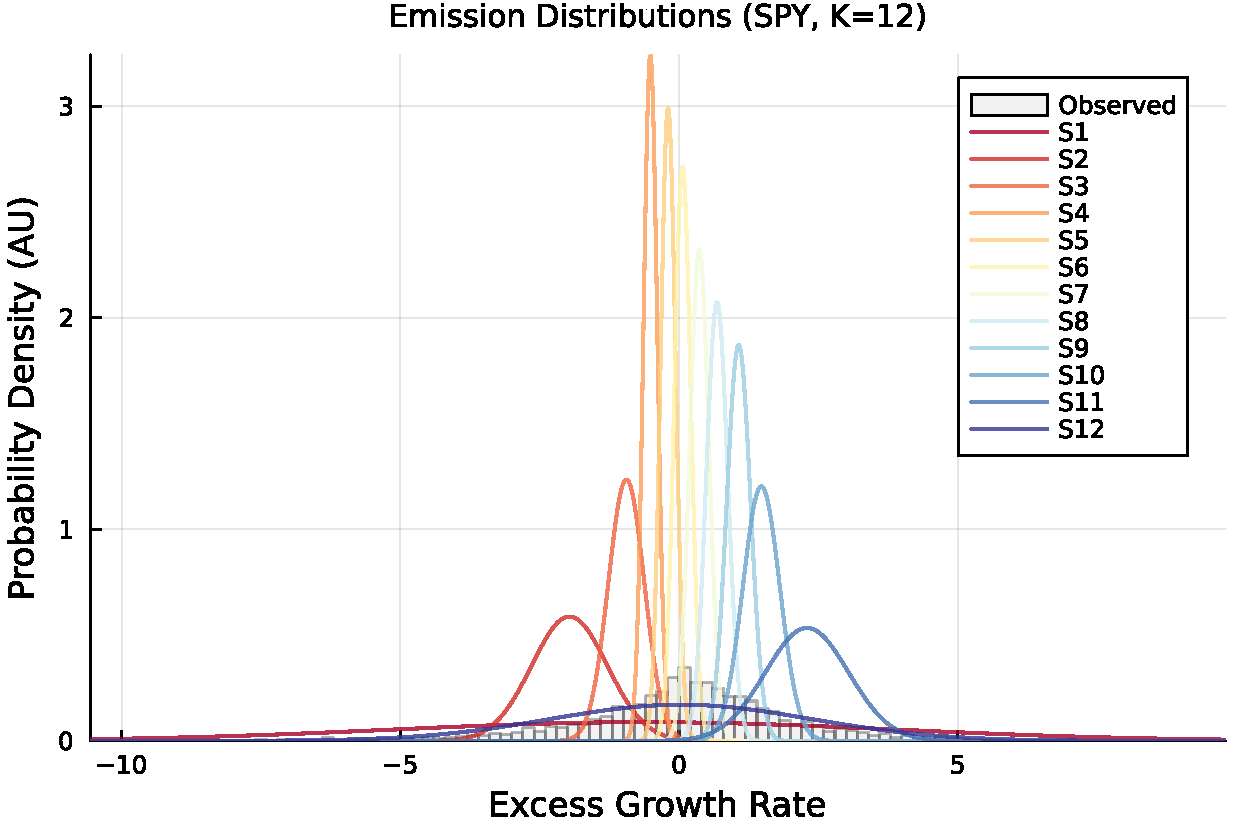
\includegraphics[width=\textwidth]{sections/figs/Fig-Emission-PDFs-K12.pdf}
    \caption{$K = 12$}
\end{subfigure}
\hfill
\begin{subfigure}[b]{0.24\textwidth}
    
\includegraphics[width=\textwidth]{sections/figs/Fig-Emission-PDFs-K18.pdf}
    \caption{$K = 18$ (selected)}
\end{subfigure}
\caption{Learned Gaussian emission distributions across state resolutions, overlaid on the observed SPY return histogram. Higher $K$ values produce finer decomposition with dedicated states capturing tail behavior.}
\label{fig:emissions_all}
\end{figure}

\subsection{Transition Matrix Structure}

Figure~\ref{fig:transition_all} shows the learned transition matrices for $K = 6$ and $K = 18$ in log$_{10}$ color scale.
Both matrices exhibit a dominant near-diagonal band, reflecting the tendency of the market to remain in its current regime.
Off-diagonal entries decay with distance from the diagonal, indicating that large regime jumps (for example, from a deep crash state directly to a boom state) are rare but nonzero.

The diagonal dominance is critical for the ACF-MAE result discussed in Section~\ref{sec:discussion}: the self-transition probabilities $T_{kk}$ for central states are typically 0.7--0.95, producing mean sojourn times of 3--20 days.
The mixture of these geometric sojourn times across states produces the sum-of-exponentials ACF profile that approximates the observed slow decay.

\begin{figure}[H]
\centering
\begin{subfigure}[b]{0.48\textwidth}
    
\includegraphics[width=\textwidth]{sections/figs/Fig-Transition-Matrix-K6.pdf}
    \caption{$K = 6$}
\end{subfigure}
\hfill
\begin{subfigure}[b]{0.48\textwidth}
    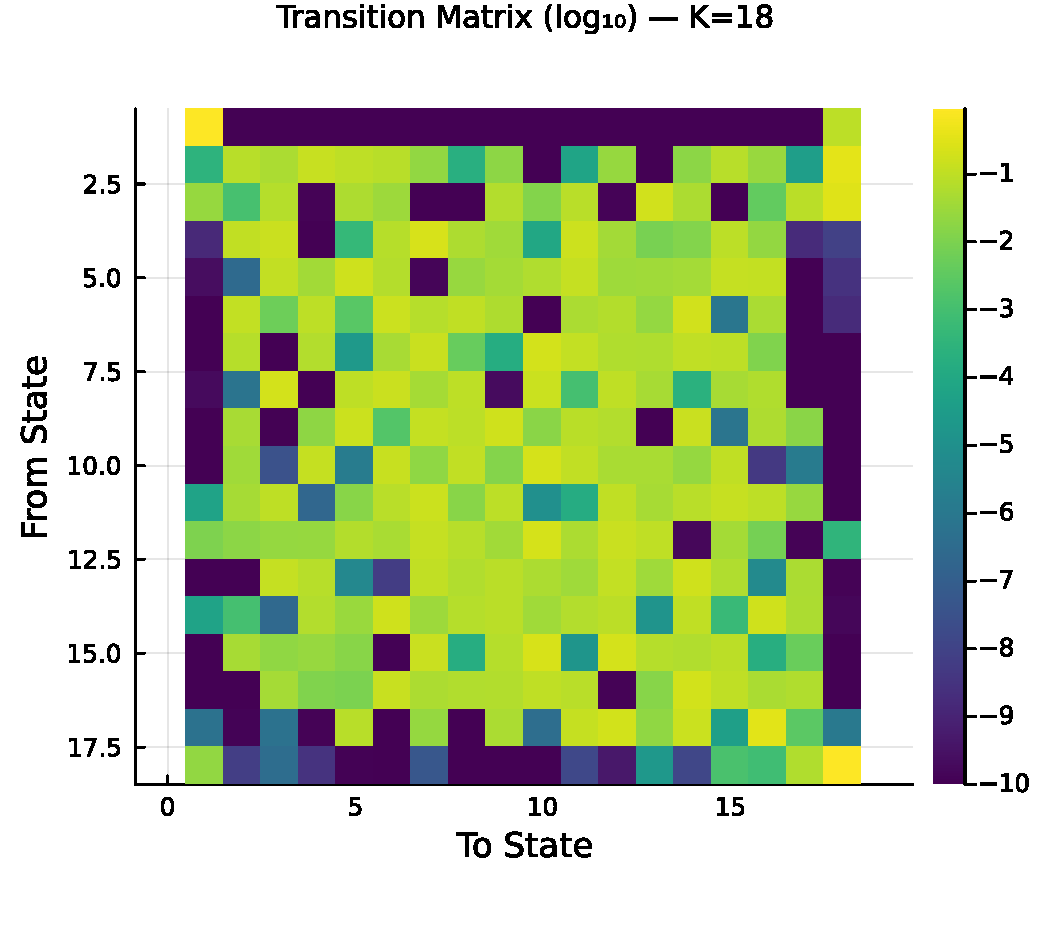
\includegraphics[width=\textwidth]{sections/figs/Fig-Transition-Matrix-K18.pdf}
    \caption{$K = 18$ (selected)}
\end{subfigure}
\caption{Learned transition matrices in log$_{10}$ color scale. The near-diagonal band reflects regime persistence; off-diagonal entries decay with distance, indicating that large regime transitions are rare.}
\label{fig:transition_all}
\end{figure}

\subsection{Stationary Distributions and Residence Times}

Figure~\ref{fig:stationary_all} shows the stationary distributions $\bar{\boldsymbol{\pi}}$ for $K = 6$ and $K = 18$.
In both cases, the central states (those with $\mu_k$ near zero and moderate $\sigma_k$) receive the highest stationary probability, consistent with the empirical concentration of returns near zero.
Tail states (crash and boom) receive low stationary probability, consistent with the rarity of extreme events.

Figure~\ref{fig:residence_all} shows the natural residence times $\tau_k = 1/(1 - T_{kk})$ per state for $K = 6$ and $K = 18$.
Under pure Markov dynamics (no jump mechanism), the expected duration in state $k$ before transitioning is $\tau_k$ steps.
Central states exhibit the longest residence times (5--20 days), while tail states have shorter residence times (1--3 days), consistent with the transient nature of extreme market events.
Notably, even without a jump mechanism, the tail states at higher $K$ maintain sufficient self-transition probability ($T_{kk} \approx 0.3$--$0.5$) to produce multi-day tail episodes.
This contrasts with the discrete model of \citet{alswaidan2026hybrid}, where tail-state residence times were too short to sustain clustering without the Poisson jump extension.

\begin{figure}[H]
\centering
\begin{subfigure}[b]{0.48\textwidth}
    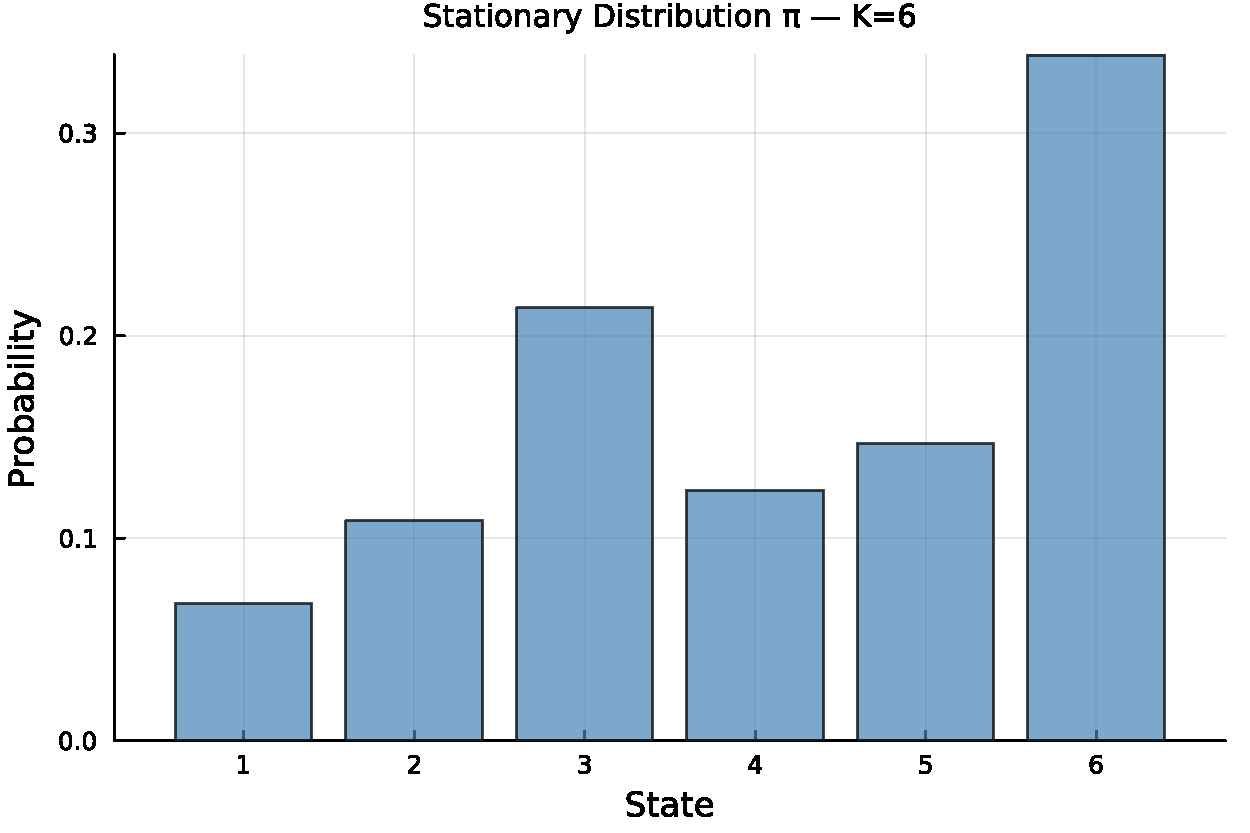
\includegraphics[width=\textwidth]{sections/figs/Fig-Stationary-Distribution-K6.pdf}
    \caption{$K = 6$}
\end{subfigure}
\hfill
\begin{subfigure}[b]{0.48\textwidth}
    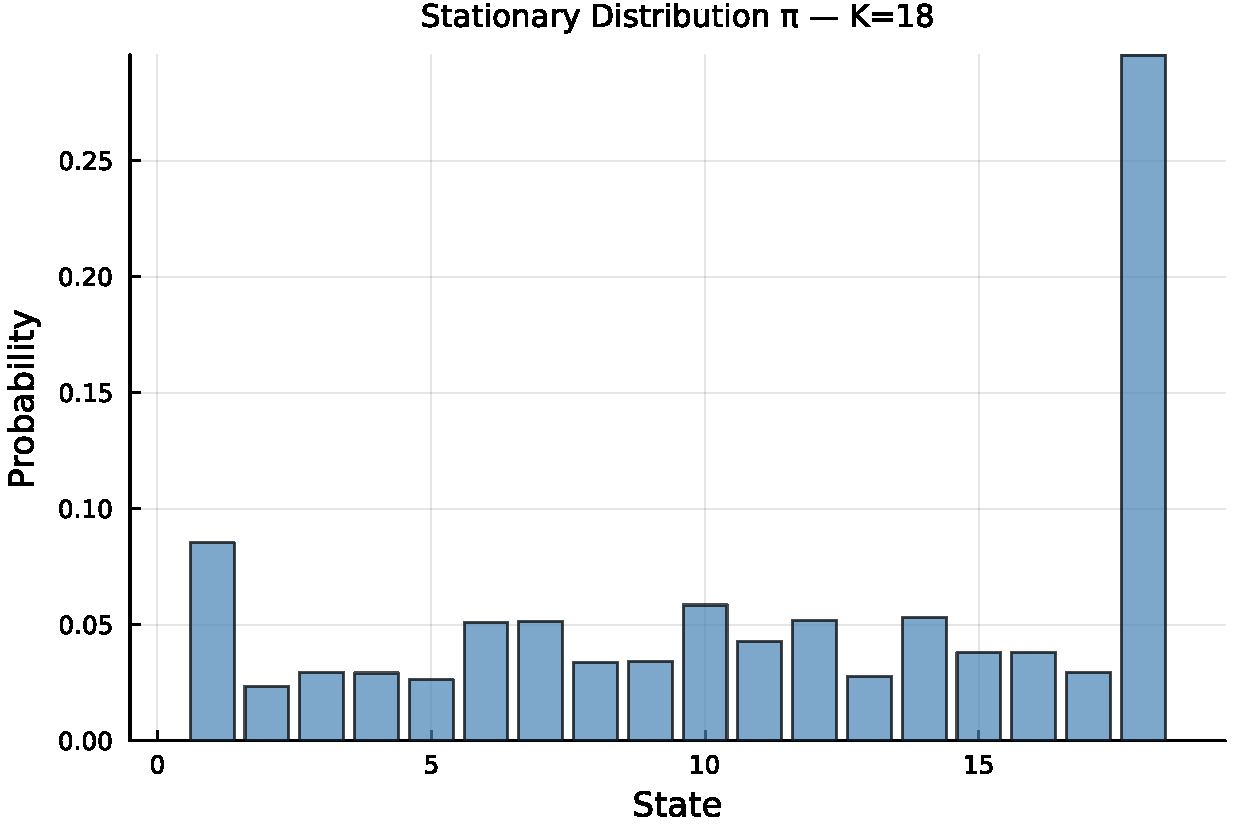
\includegraphics[width=\textwidth]{sections/figs/Fig-Stationary-Distribution-K18.pdf}
    \caption{$K = 18$}
\end{subfigure}
\caption{Stationary distributions $\bar{\boldsymbol{\pi}}$ for $K = 6$ and $K = 18$. Central states receive the highest stationary probability, consistent with the concentration of returns near zero.}
\label{fig:stationary_all}
\end{figure}

\begin{figure}[H]
\centering
\begin{subfigure}[b]{0.48\textwidth}
    
\includegraphics[width=\textwidth]{sections/figs/Fig-Residence-Times-K6.pdf}
    \caption{$K = 6$}
\end{subfigure}
\hfill
\begin{subfigure}[b]{0.48\textwidth}
    
\includegraphics[width=\textwidth]{sections/figs/Fig-Residence-Times-K18.pdf}
    \caption{$K = 18$}
\end{subfigure}
\caption{Natural residence times $\tau_k = 1/(1 - T_{kk})$ per state. Central states have the longest residence times (5--20 days), while tail states are shorter-lived (1--3 days). This asymmetry drives volatility clustering.}
\label{fig:residence_all}
\end{figure}

\subsection{In-Sample Comparison at Non-Selected State Resolutions}
\label{sec:k_sweep_panels}

Figure~\ref{fig:k_sweep_panels_is} shows the in-sample model comparison panels for $K \in \{3, 6, 9, 12, 15, 21\}$, complementing the $K = 18$ comparison in Figure~\ref{fig:is_comparison} of the main text.
Across all resolutions, the CHMM's simulated density closely overlays the observed density, and the ACF of absolute returns tracks the slow decay pattern.
The visible improvement from $K = 3$ to $K = 18$ is concentrated in the tails of the Q-Q panel and the steady-state level of the ACF panel.

\begin{figure}[H]
\centering
\begin{subfigure}[b]{0.32\textwidth}
    
\includegraphics[width=\textwidth]{sections/figs/Fig-3-IS-Comparison-K3.pdf}
    \caption{$K = 3$}
\end{subfigure}
\hfill
\begin{subfigure}[b]{0.32\textwidth}
    
\includegraphics[width=\textwidth]{sections/figs/Fig-3-IS-Comparison-K6.pdf}
    \caption{$K = 6$}
\end{subfigure}
\hfill
\begin{subfigure}[b]{0.32\textwidth}
    
\includegraphics[width=\textwidth]{sections/figs/Fig-3-IS-Comparison-K9.pdf}
    \caption{$K = 9$}
\end{subfigure}

\vspace{0.4cm}

\begin{subfigure}[b]{0.32\textwidth}
    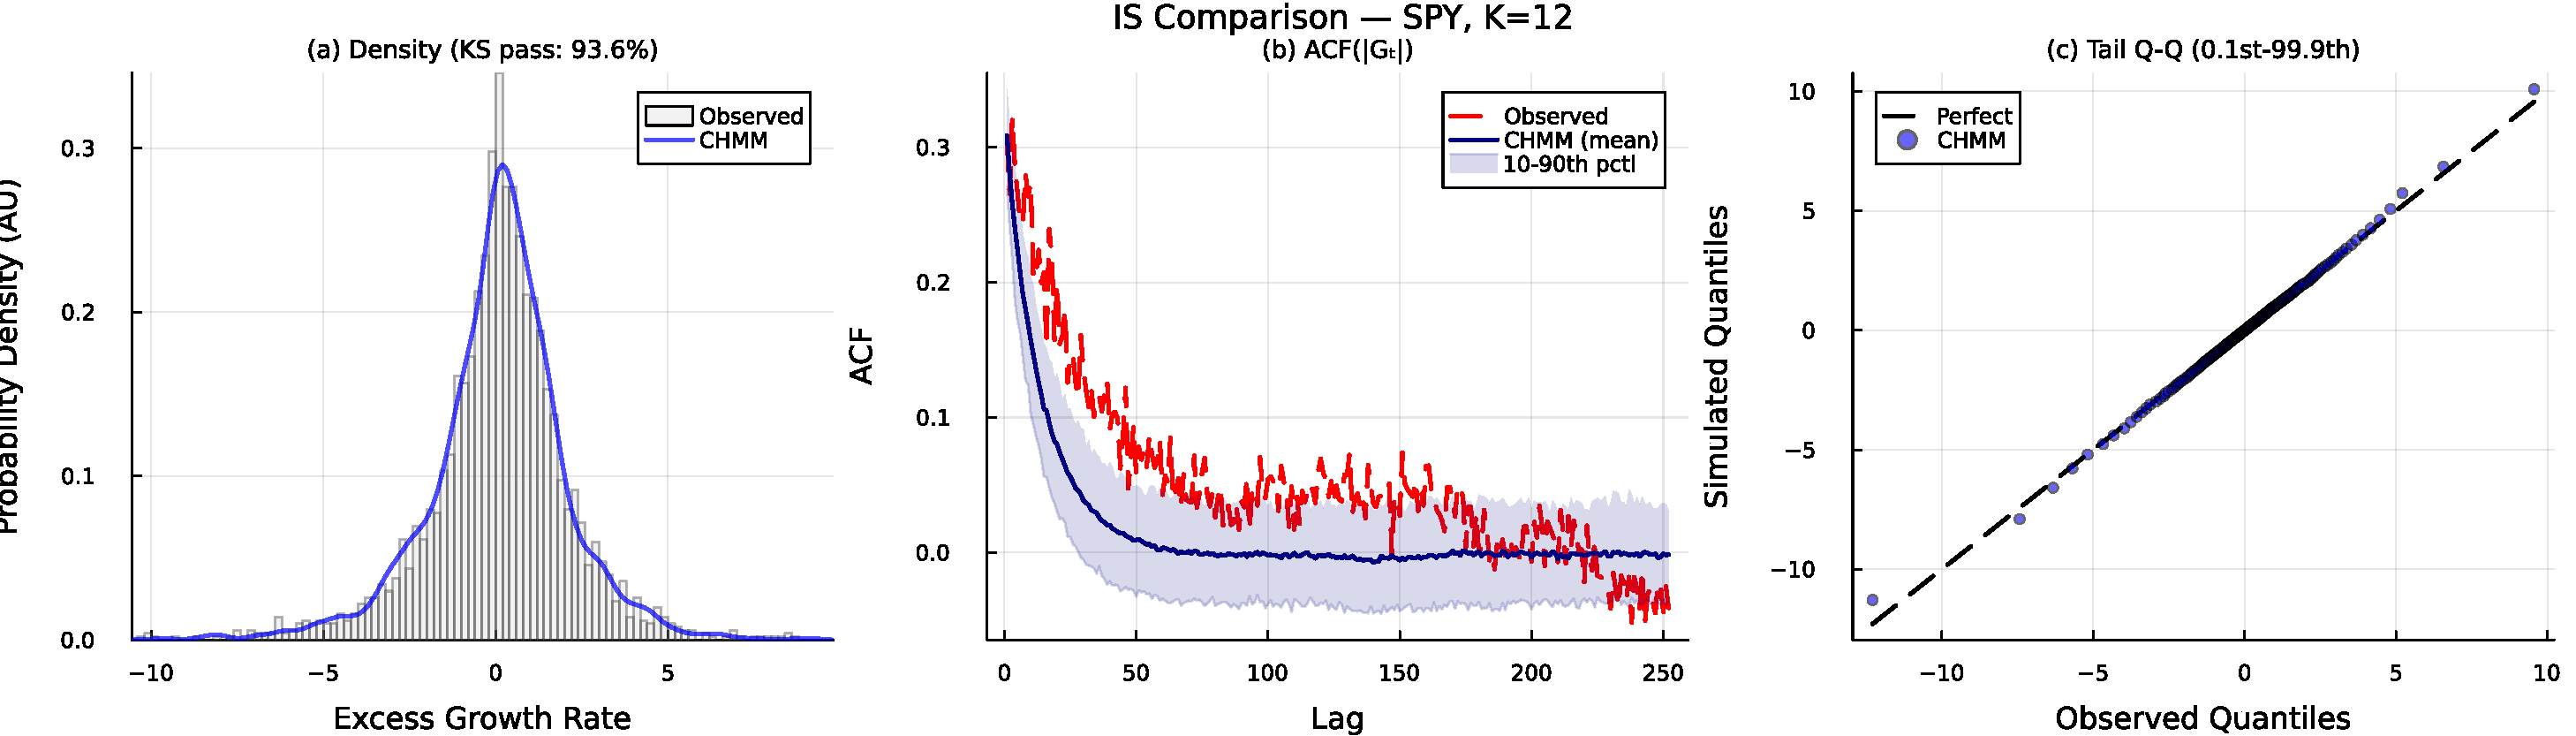
\includegraphics[width=\textwidth]{sections/figs/Fig-3-IS-Comparison-K12.pdf}
    \caption{$K = 12$}
\end{subfigure}
\hfill
\begin{subfigure}[b]{0.32\textwidth}
    
\includegraphics[width=\textwidth]{sections/figs/Fig-3-IS-Comparison-K15.pdf}
    \caption{$K = 15$}
\end{subfigure}
\hfill
\begin{subfigure}[b]{0.32\textwidth}
    
\includegraphics[width=\textwidth]{sections/figs/Fig-3-IS-Comparison-K21.pdf}
    \caption{$K = 21$}
\end{subfigure}
\caption{In-sample CHMM comparison panels at the non-selected state resolutions. Panel $K = 18$ is reproduced in Figure~\ref{fig:is_comparison} of the main text.}
\label{fig:k_sweep_panels_is}
\end{figure}

\subsection{Out-of-Sample Validation at Non-Selected State Resolutions}

Figure~\ref{fig:k_sweep_panels_oos} shows the out-of-sample validation panels for $K \in \{3, 6, 9, 12, 15, 21\}$.
KS pass rates remain above 91\% at all resolutions; the $K = 18$ panel is reproduced in Figure~\ref{fig:oos_validation} of the main text.

\begin{figure}[H]
\centering
\begin{subfigure}[b]{0.32\textwidth}
    
\includegraphics[width=\textwidth]{sections/figs/Fig-4-OoS-Validation-K3.pdf}
    \caption{$K = 3$}
\end{subfigure}
\hfill
\begin{subfigure}[b]{0.32\textwidth}
    
\includegraphics[width=\textwidth]{sections/figs/Fig-4-OoS-Validation-K6.pdf}
    \caption{$K = 6$}
\end{subfigure}
\hfill
\begin{subfigure}[b]{0.32\textwidth}
    
\includegraphics[width=\textwidth]{sections/figs/Fig-4-OoS-Validation-K9.pdf}
    \caption{$K = 9$}
\end{subfigure}

\vspace{0.4cm}

\begin{subfigure}[b]{0.32\textwidth}
    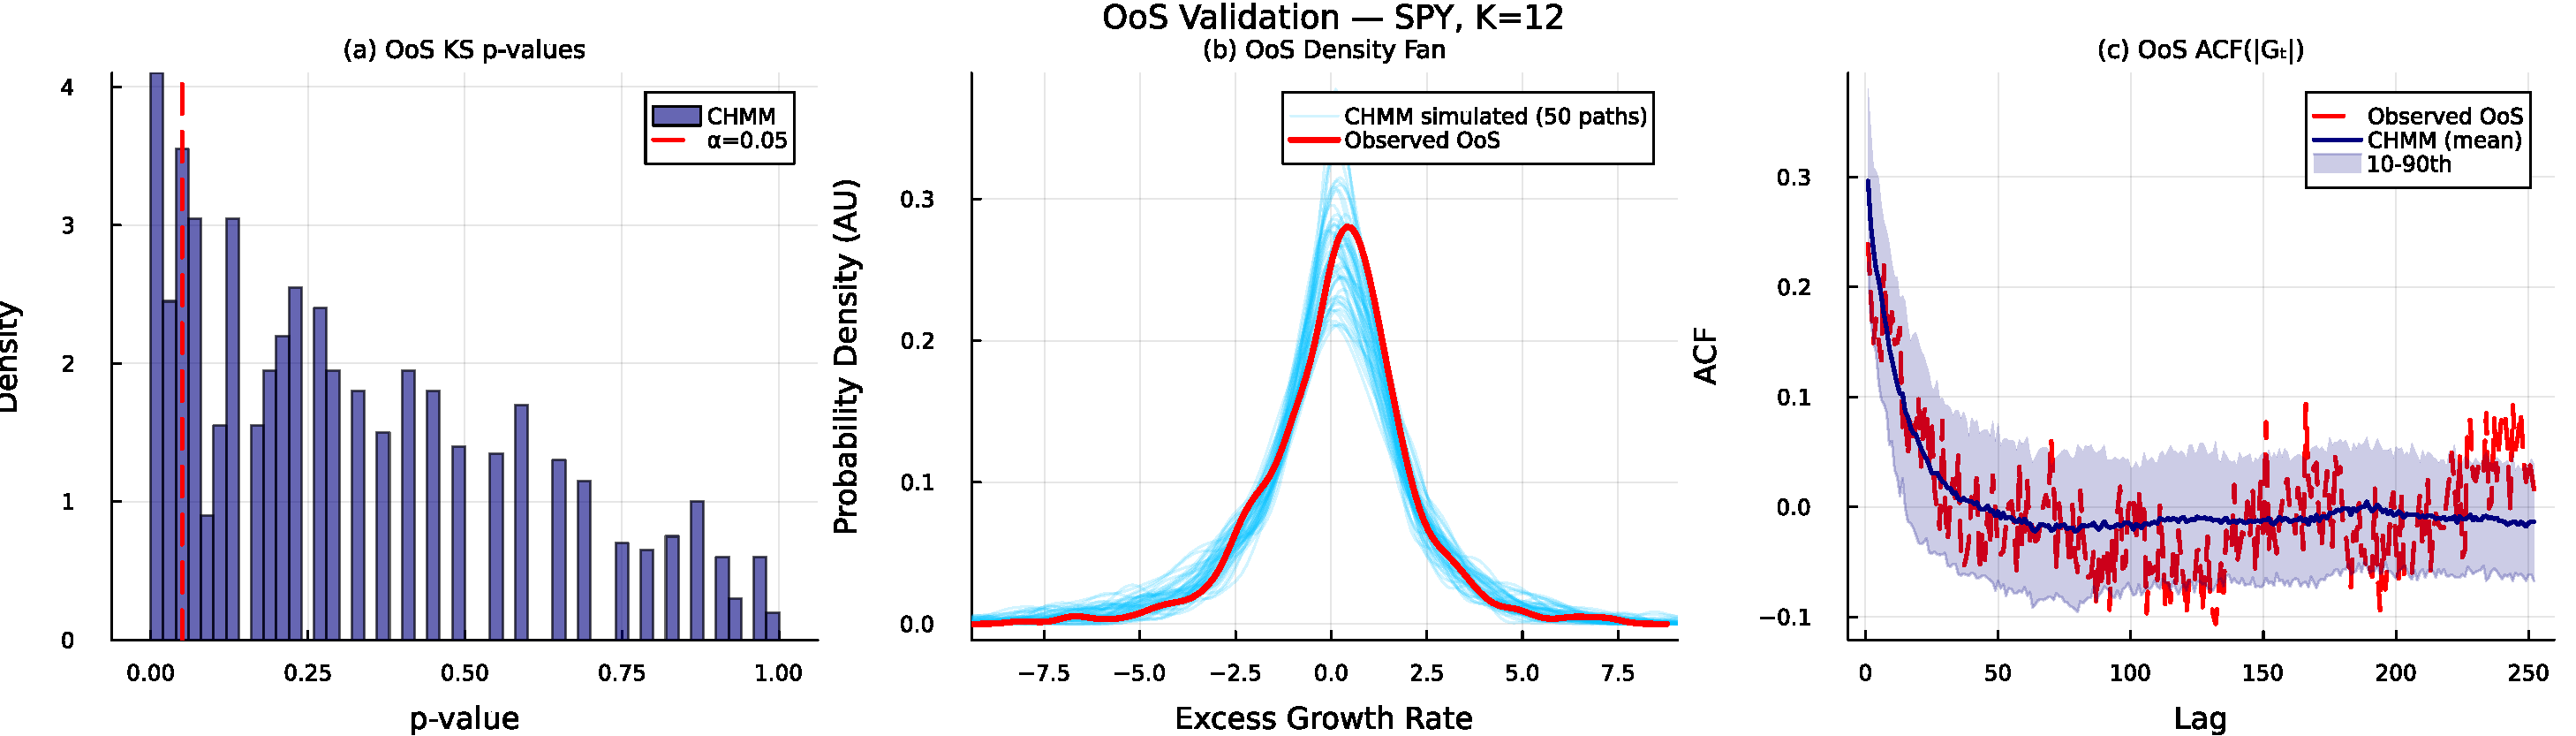
\includegraphics[width=\textwidth]{sections/figs/Fig-4-OoS-Validation-K12.pdf}
    \caption{$K = 12$}
\end{subfigure}
\hfill
\begin{subfigure}[b]{0.32\textwidth}
    
\includegraphics[width=\textwidth]{sections/figs/Fig-4-OoS-Validation-K15.pdf}
    \caption{$K = 15$}
\end{subfigure}
\hfill
\begin{subfigure}[b]{0.32\textwidth}
    
\includegraphics[width=\textwidth]{sections/figs/Fig-4-OoS-Validation-K21.pdf}
    \caption{$K = 21$}
\end{subfigure}
\caption{Out-of-sample CHMM validation panels at the non-selected state resolutions.}
\label{fig:k_sweep_panels_oos}
\end{figure}

\subsection{ACF Comparison Across State Resolutions}

Figure~\ref{fig:acf_all} shows the ACF of $|G_t|$ for the CHMM at $K = 3$, $K = 12$, and $K = 18$, compared to the observed ACF.
At all resolutions, the simulated ACF (shown as the median with 10th--90th percentile envelope across 1{,}000 paths) tracks the observed slow decay pattern.

\begin{figure}[H]
\centering
\begin{subfigure}[b]{0.32\textwidth}
    
\includegraphics[width=\textwidth]{sections/figs/Fig-ACF-Comparison-K3.pdf}
    \caption{$K = 3$}
\end{subfigure}
\hfill
\begin{subfigure}[b]{0.32\textwidth}
    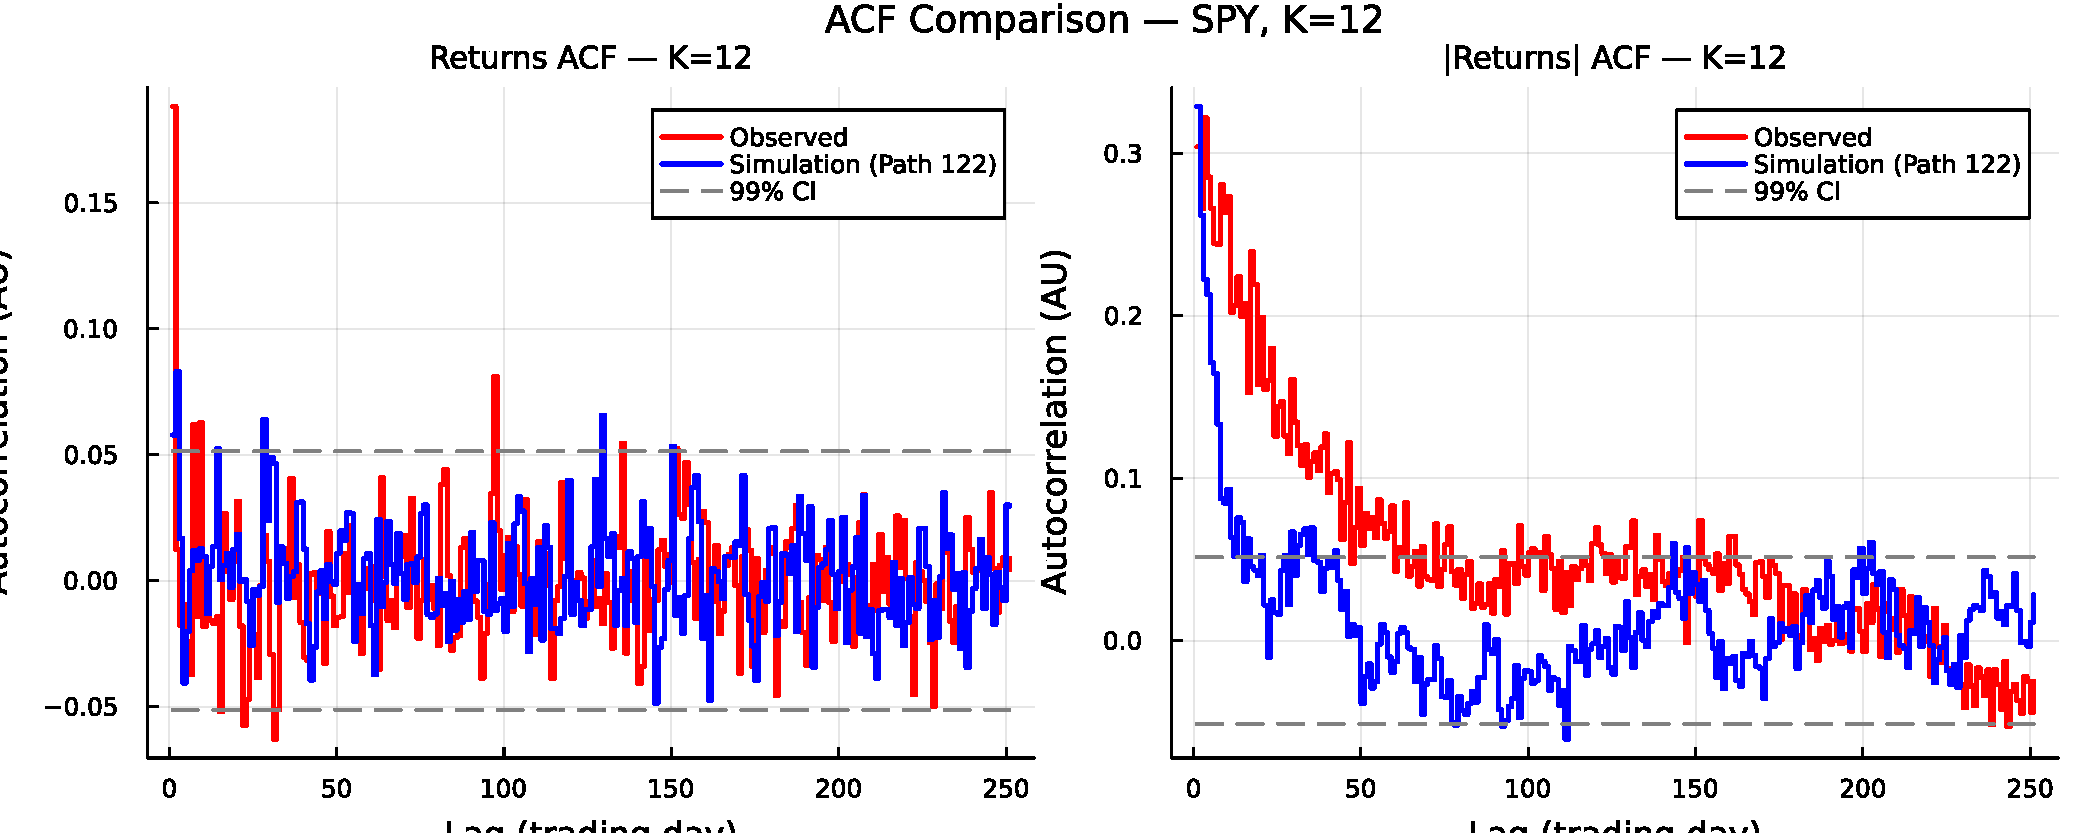
\includegraphics[width=\textwidth]{sections/figs/Fig-ACF-Comparison-K12.pdf}
    \caption{$K = 12$}
\end{subfigure}
\hfill
\begin{subfigure}[b]{0.32\textwidth}
    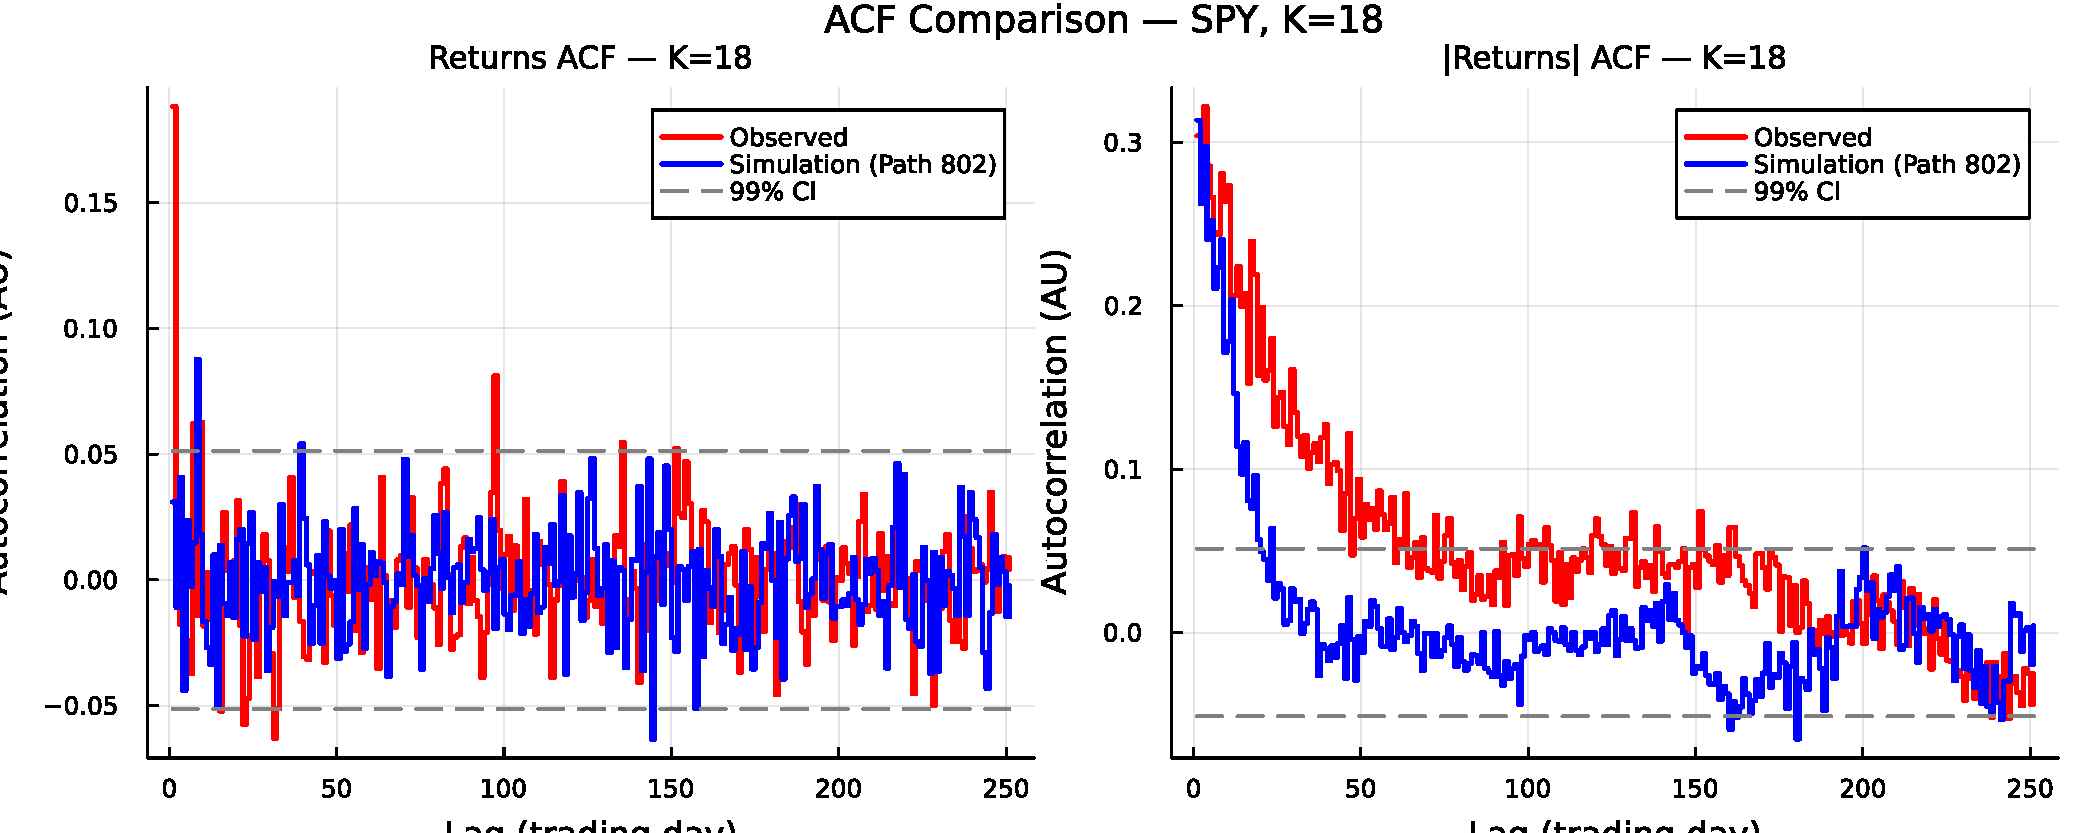
\includegraphics[width=\textwidth]{sections/figs/Fig-ACF-Comparison-K18.pdf}
    \caption{$K = 18$ (selected)}
\end{subfigure}
\caption{ACF of $|G_t|$ for the CHMM at $K = 3$, $K = 12$, and $K = 18$. The simulated 10th--90th percentile envelope (shaded) envelopes the observed ACF (red dashed), confirming that the CHMM reproduces volatility clustering without jump augmentation across the entire sweep.}
\label{fig:acf_all}
\end{figure}

\subsection{Example Simulated Trajectories}

Figure~\ref{fig:trajectories} shows example simulated return trajectories for $K = 6$ and $K = 18$, illustrating the qualitative dynamics produced by the CHMM.
Both trajectories exhibit the characteristic pattern of financial returns: extended periods of low volatility punctuated by clusters of large-magnitude events.

\begin{figure}[H]
\centering
\begin{subfigure}[b]{0.48\textwidth}
    
\includegraphics[width=\textwidth]{sections/figs/Fig-Trajectory-Example-K6.pdf}
    \caption{$K = 6$}
\end{subfigure}
\hfill
\begin{subfigure}[b]{0.48\textwidth}
    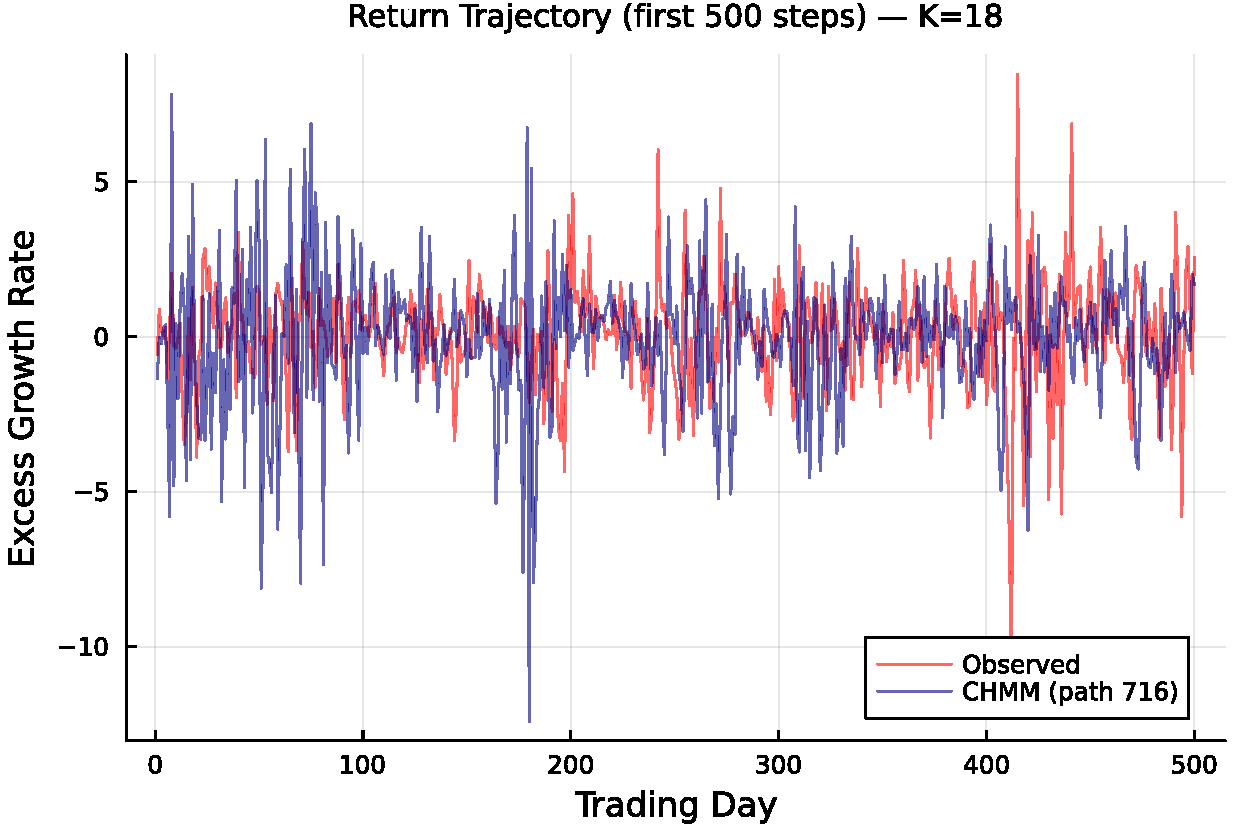
\includegraphics[width=\textwidth]{sections/figs/Fig-Trajectory-Example-K18.pdf}
    \caption{$K = 18$}
\end{subfigure}
\caption{Example simulated return trajectories. The alternation between calm (central states) and volatile (tail states) periods produces the volatility clustering characteristic of empirical financial returns.}
\label{fig:trajectories}
\end{figure}

\subsection{Multi-Emission Figures at $K = 18$}
\label{sec:multi_emission_figs}

This appendix reproduces the standard diagnostic suite (emission PDFs, transition matrix, stationary distribution, residence times, IS comparison, OoS validation, and convergence) for the two heavy-tailed emission families (CHMM-t and CHMM-L) at the selected state resolution $K = 18$.
The Gaussian counterparts are already shown as Figures~\ref{fig:model_internals},~\ref{fig:is_comparison},~\ref{fig:oos_validation},~\ref{fig:convergence_all},~\ref{fig:transition_all},~\ref{fig:stationary_all}, and~\ref{fig:residence_all} in the main text and above in this appendix.
The figures confirm that the shared forward--backward scaffold produces internally-similar regime structure across the three families: the near-diagonal transition band, the $K$-component dense emission cover, the longer central-state residence times, and the monotone log-likelihood convergence are features of the CHMM framework and not of the Gaussian component specifically.

\paragraph{Emission PDFs.}
Figure~\ref{fig:emissions_families} compares the learned $K = 18$ emissions for the three families.
The CHMM-t panel's per-state $\nu_k$ allocation is visible in the narrower modes of certain tail states; the CHMM-L panel's Laplace components have sharper peaks and slower exponential tail decay than the Gaussians.

\begin{figure}[H]
\centering
\begin{subfigure}[b]{0.32\textwidth}
    
\includegraphics[width=\textwidth]{sections/figs/Fig-Emission-PDFs-K18-N.pdf}
    \caption{CHMM-N (Gaussian)}
\end{subfigure}
\hfill
\begin{subfigure}[b]{0.32\textwidth}
    
\includegraphics[width=\textwidth]{sections/figs/Fig-Emission-PDFs-K18-t.pdf}
    \caption{CHMM-t (Student-t)}
\end{subfigure}
\hfill
\begin{subfigure}[b]{0.32\textwidth}
    
\includegraphics[width=\textwidth]{sections/figs/Fig-Emission-PDFs-K18-L.pdf}
    \caption{CHMM-L (Laplace)}
\end{subfigure}
\caption{Learned emission distributions at $K = 18$ across the three emission families, overlaid on the observed SPY return histogram. Heavier-tailed emission families (t, L) give individual components more tail mass, which is what closes the kurtosis gap of the Gaussian CHMM.}
\label{fig:emissions_families}
\end{figure}

\paragraph{Transition matrices.}
Figure~\ref{fig:transition_families} shows the $K = 18$ transition matrices learned by each family.
The near-diagonal band and the magnitude of self-transition probabilities are essentially unchanged across families, consistent with the ACF-MAE being stable across the family axis (Table~\ref{tab:sensitivity_multi}).

\begin{figure}[H]
\centering
\begin{subfigure}[b]{0.32\textwidth}
    
\includegraphics[width=\textwidth]{sections/figs/Fig-Transition-Matrix-K18-N.pdf}
    \caption{CHMM-N}
\end{subfigure}
\hfill
\begin{subfigure}[b]{0.32\textwidth}
    
\includegraphics[width=\textwidth]{sections/figs/Fig-Transition-Matrix-K18-t.pdf}
    \caption{CHMM-t}
\end{subfigure}
\hfill
\begin{subfigure}[b]{0.32\textwidth}
    
\includegraphics[width=\textwidth]{sections/figs/Fig-Transition-Matrix-K18-L.pdf}
    \caption{CHMM-L}
\end{subfigure}
\caption{Learned transition matrices at $K = 18$ in log$_{10}$ color scale. The diagonal-band structure is preserved across all three emission families.}
\label{fig:transition_families}
\end{figure}

\paragraph{Stationary distributions and residence times.}
Figure~\ref{fig:stationary_families} and Figure~\ref{fig:residence_families} compare the stationary distribution and natural residence times $\tau_k = 1/(1 - T_{kk})$ across families at $K = 18$.
The mass concentration at central states and the monotone decrease of $\tau_k$ toward the tails are features of the regime structure, not the emission family.

\begin{figure}[H]
\centering
\begin{subfigure}[b]{0.32\textwidth}
    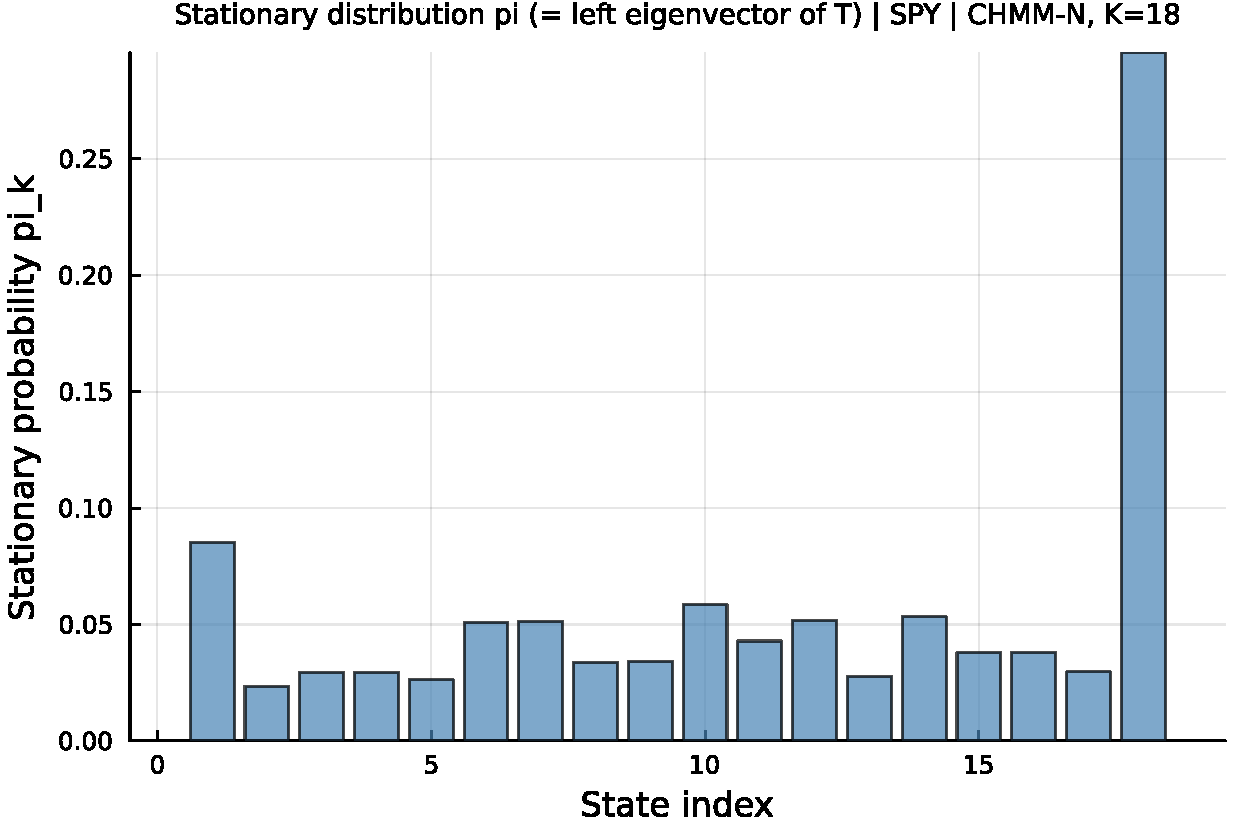
\includegraphics[width=\textwidth]{sections/figs/Fig-Stationary-Distribution-K18-N.pdf}
    \caption{CHMM-N}
\end{subfigure}
\hfill
\begin{subfigure}[b]{0.32\textwidth}
    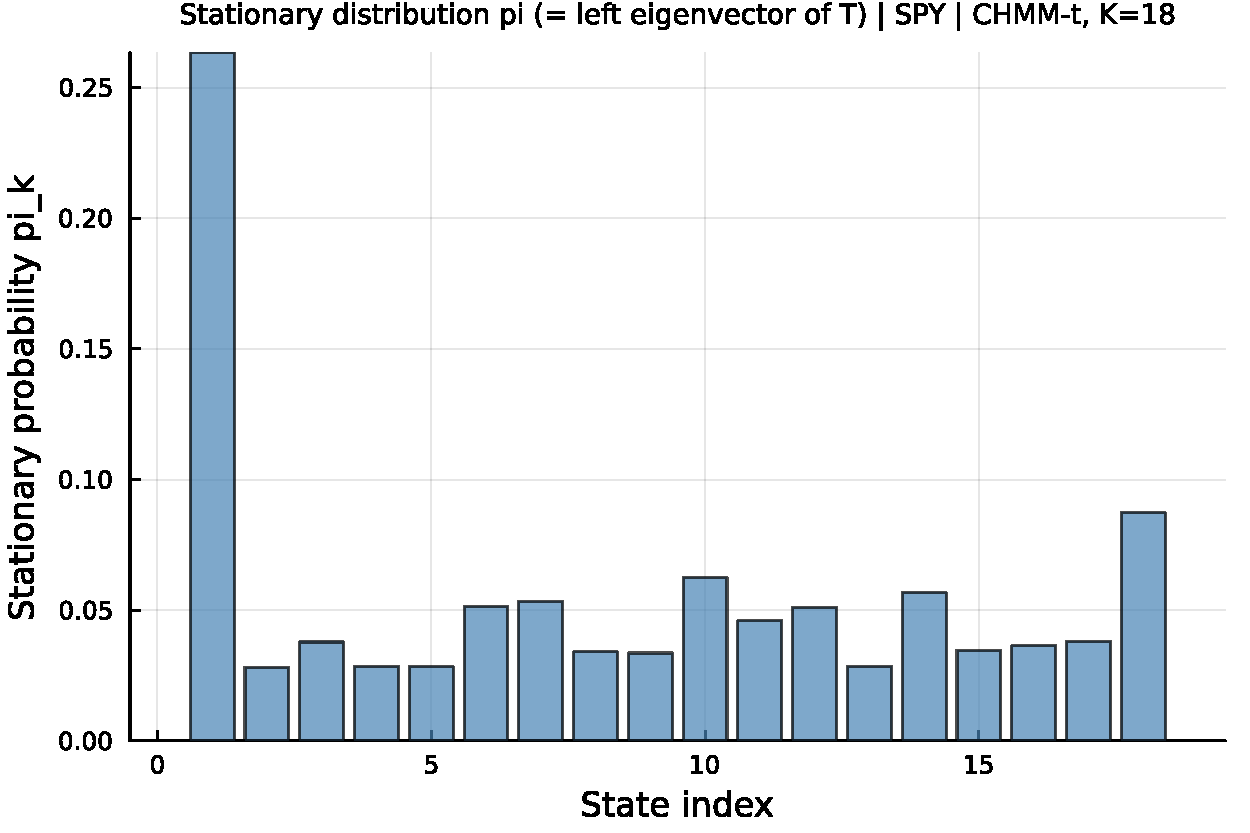
\includegraphics[width=\textwidth]{sections/figs/Fig-Stationary-Distribution-K18-t.pdf}
    \caption{CHMM-t}
\end{subfigure}
\hfill
\begin{subfigure}[b]{0.32\textwidth}
    
\includegraphics[width=\textwidth]{sections/figs/Fig-Stationary-Distribution-K18-L.pdf}
    \caption{CHMM-L}
\end{subfigure}
\caption{Stationary distributions $\bar{\boldsymbol{\pi}}$ at $K = 18$ across the three emission families.}
\label{fig:stationary_families}
\end{figure}

\begin{figure}[H]
\centering
\begin{subfigure}[b]{0.32\textwidth}
    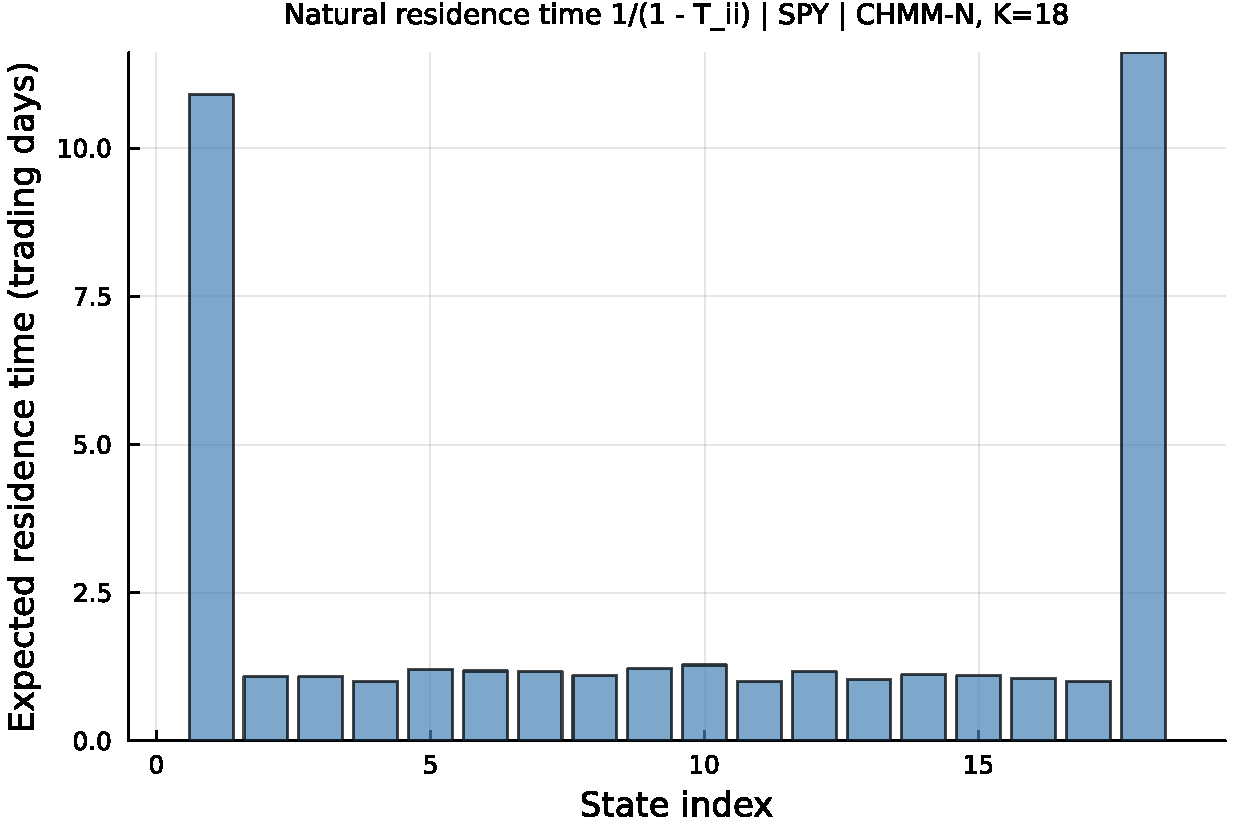
\includegraphics[width=\textwidth]{sections/figs/Fig-Residence-Times-K18-N.pdf}
    \caption{CHMM-N}
\end{subfigure}
\hfill
\begin{subfigure}[b]{0.32\textwidth}
    
\includegraphics[width=\textwidth]{sections/figs/Fig-Residence-Times-K18-t.pdf}
    \caption{CHMM-t}
\end{subfigure}
\hfill
\begin{subfigure}[b]{0.32\textwidth}
    
\includegraphics[width=\textwidth]{sections/figs/Fig-Residence-Times-K18-L.pdf}
    \caption{CHMM-L}
\end{subfigure}
\caption{Natural residence times $\tau_k = 1/(1 - T_{kk})$ at $K = 18$ across the three emission families.}
\label{fig:residence_families}
\end{figure}

\paragraph{In-sample comparison.}
Figure~\ref{fig:is_families} reproduces the three-panel in-sample comparison (density, ACF of $|G_t|$, tail Q-Q) at $K = 18$ for the two heavy-tailed families; the CHMM-N panel is Figure~\ref{fig:is_comparison} in the main text.

\begin{figure}[H]
\centering
\begin{subfigure}[b]{0.48\textwidth}
    
\includegraphics[width=\textwidth]{sections/figs/Fig-3-IS-Comparison-K18-t.pdf}
    \caption{CHMM-t}
\end{subfigure}
\hfill
\begin{subfigure}[b]{0.48\textwidth}
    
\includegraphics[width=\textwidth]{sections/figs/Fig-3-IS-Comparison-K18-L.pdf}
    \caption{CHMM-L}
\end{subfigure}
\caption{In-sample model comparison at $K = 18$ for the two heavy-tailed emission families. Each panel shows (a) marginal density with KS pass rate, (b) ACF of $|G_t|$, and (c) tail Q-Q plot. The CHMM-N counterpart is Figure~\ref{fig:is_comparison}.}
\label{fig:is_families}
\end{figure}

\paragraph{Out-of-sample validation.}
Figure~\ref{fig:oos_families} shows the OoS validation panels for CHMM-t and CHMM-L at $K = 18$.
The CHMM-t panel demonstrates the OoS kurtosis alignment noted in the main text (simulated 6.40 vs.\ observed 6.24), and the CHMM-L panel shows the tighter density fan produced by the heavier Laplace tails relative to the Gaussian.

\begin{figure}[H]
\centering
\begin{subfigure}[b]{0.48\textwidth}
    
\includegraphics[width=\textwidth]{sections/figs/Fig-4-OoS-Validation-K18-t.pdf}
    \caption{CHMM-t}
\end{subfigure}
\hfill
\begin{subfigure}[b]{0.48\textwidth}
    
\includegraphics[width=\textwidth]{sections/figs/Fig-4-OoS-Validation-K18-L.pdf}
    \caption{CHMM-L}
\end{subfigure}
\caption{Out-of-sample validation at $K = 18$ for the two heavy-tailed emission families. Each panel shows (a) KS $p$-values, (b) OoS density fan, and (c) OoS ACF of $|G_t|$. The CHMM-N counterpart is Figure~\ref{fig:oos_validation}.}
\label{fig:oos_families}
\end{figure}

\paragraph{Convergence.}
Figure~\ref{fig:convergence_families} shows the Baum-Welch / ECM / weighted-EM log-likelihood histories at $K = 18$ for all three families.
The CHMM-t and CHMM-L curves inherit the monotone increase of the classical EM guarantee; the CHMM-t curve has a slightly longer pre-plateau phase because each ECM sub-iteration refines $\nu_k$ with a golden-section search.

\begin{figure}[H]
\centering
\begin{subfigure}[b]{0.32\textwidth}
    
\includegraphics[width=\textwidth]{sections/figs/Fig-Convergence-K18-N.pdf}
    \caption{CHMM-N}
\end{subfigure}
\hfill
\begin{subfigure}[b]{0.32\textwidth}
    
\includegraphics[width=\textwidth]{sections/figs/Fig-Convergence-K18-t.pdf}
    \caption{CHMM-t}
\end{subfigure}
\hfill
\begin{subfigure}[b]{0.32\textwidth}
    
\includegraphics[width=\textwidth]{sections/figs/Fig-Convergence-K18-L.pdf}
    \caption{CHMM-L}
\end{subfigure}
\caption{Log-likelihood histories at $K = 18$ across the three emission families. All three curves are monotonically non-decreasing and plateau well before the $\texttt{max\_iter} = 60$ budget.}
\label{fig:convergence_families}
\end{figure}

\subsection{Cross-Asset Dependence Models: Derivations and Diagnostics}
\label{sec:cross_asset_supp}

This appendix provides the technical background for the SIM and copula constructions used in Section~\ref{sec:cross_asset} of the main text.

\paragraph{Sklar's theorem and the rank-reordering simulator.}
Sklar's theorem \cite{sklar1959fonctions, nelsen2006introduction} states that any $d$-dimensional joint CDF $H(g_1, \dots, g_d)$ with continuous marginals $F_1, \dots, F_d$ can be written as $H = C(F_1, \dots, F_d)$ for a unique copula $C$.
The rank-reordering simulator exploits this uniqueness.
If $\tilde{\mathbf{G}}$ is a matrix whose $j$-th column is an i.i.d.\ sample from $F_j$, and $\mathbf{U}$ is an independent sample from $C$, then reordering each column of $\tilde{\mathbf{G}}$ so that its ranks match $\mathbf{U}$'s produces a sample from $H$, up to discrete approximation error in the empirical ranks.
Crucially, reordering never creates new values: each column of the output is a permutation of the corresponding column of $\tilde{\mathbf{G}}$, so marginal distributions are preserved exactly \cite{iman1982distribution}.

\paragraph{Kendall's $\tau$ inversion.}
Given in-sample returns $\mathbf{R} \in \mathbb{R}^{T \times d}$, we estimate the pairwise Kendall's $\tau_{ij}$ from concordant/discordant pair counts and invert to the correlation scale via the analytic relationship $\rho_{ij} = \sin(\pi \tau_{ij} / 2)$, which holds exactly for the Gaussian copula family and is commonly used as a robust correlation estimator for the Student-t copula \cite{embrechts2002correlation, mcneil2015quantitative}.
The resulting matrix $\hat{\Sigma}$ is symmetric but not guaranteed positive semi-definite; we project to the nearest PSD matrix by clipping negative eigenvalues to $10^{-8}$ and rescaling the diagonal to unity.

\paragraph{Profile MLE for $\nu$.}
The Student-t copula log-density at a single pseudo-uniform observation $\mathbf{u} \in [0,1]^d$, with $x_j = t_\nu^{-1}(u_j)$ and $\mathbf{x} = (x_1, \dots, x_d)^\top$, is
\begin{align}
    \log c_t(\mathbf{u}; \Sigma, \nu)
    \;=\;&
    \log \Gamma\!\left(\tfrac{\nu+d}{2}\right)
    + (d-1)\,\log \Gamma\!\left(\tfrac{\nu}{2}\right)
    - d\,\log \Gamma\!\left(\tfrac{\nu+1}{2}\right)
    - \tfrac{1}{2} \log |\Sigma|
    \notag \\
    &\;
    - \tfrac{\nu+d}{2}\,\log\!\left(1 + \tfrac{\mathbf{x}^{\!\top} \Sigma^{-1} \mathbf{x}}{\nu}\right)
    + \sum_{j=1}^{d} \tfrac{\nu+1}{2}\,\log\!\left(1 + \tfrac{x_j^2}{\nu}\right).
    \label{eq:tcop_ll}
\end{align}
Summing over $t = 1, \dots, T$ pseudo-observations yields the profile log-likelihood as a function of $\nu$ with $\Sigma$ held fixed at the Kendall's-$\tau$ estimate.
We evaluate equation~\eqref{eq:tcop_ll} on the discrete grid $\nu \in \{2, 3, 4, 5, 6, 8, 10, 15, 20, 30\}$ and select $\hat{\nu}$ as the grid point with the largest total log-likelihood.
In Section~\ref{sec:cross_asset} the selected value was $\hat{\nu} = 6$ on the six-asset universe.

\paragraph{Sampling the copula.}
To sample $T$ rows from the $d$-dimensional Gaussian copula with correlation $\Sigma$, we (i) compute the Cholesky factor $\Sigma = L L^\top$, (ii) draw $Z \sim \mathcal{N}(0, I_d)$ i.i.d.\ and form $Y = L Z$, and (iii) return $U = \Phi(Y)$ componentwise.
For the Student-t copula with degrees of freedom $\nu$, we draw $W \sim \chi^2_\nu / \nu$ independent of $Y$ and form the multivariate-$t$ variate $X = Y / \sqrt{W}$, then return $U = t_\nu(X)$ componentwise.

\paragraph{SIM regression summary.}
Table~\ref{tab:sim_regression} reports the fitted SIM regression coefficients and goodness-of-fit statistics for the non-market assets in Section~\ref{sec:cross_asset}.
QQQ's high $R^2 = 0.841$ reflects that the Nasdaq-100 ETF is essentially a linear combination of large-cap technology names that also drive the S\&P~500 index, while JNJ's lower $R^2 = 0.225$ reflects the limited systematic exposure of low-beta healthcare stocks.
These factor loadings and residual magnitudes are what the SIM simulation in equation~\eqref{eq:sim_sim} re-injects at simulation time, and they explain the uneven per-asset KS pass rates reported in Table~\ref{tab:cross_asset_sim_copula}.

\begin{table}[H]
\centering
\caption{SIM regression $\hat{G}_{j,t} = \hat{\alpha}_j + \hat{\beta}_j G_{\text{SPY},t} + \hat{\eta}_{j,t}$ for the five non-market assets, fitted on the 2014--2024 in-sample window ($T = 2{,}766$). Coefficients $\hat{\alpha}, \hat{\beta}$ and $R^2$ are reported for the factor equation used in equation~\eqref{eq:sim_sim}.}
\label{tab:sim_regression}
\small
\begin{tabular}{l ccc}
\toprule
Ticker & $\hat{\alpha}$ & $\hat{\beta}$ & $R^2$ \\
\midrule
NVDA & $0.347$   & $1.749$ & $0.370$ \\
JNJ  & $-0.016$  & $0.539$ & $0.225$ \\
JPM  & $0.001$   & $1.204$ & $0.483$ \\
AAPL & $0.106$   & $1.194$ & $0.474$ \\
QQQ  & $0.041$   & $1.134$ & $0.841$ \\
\bottomrule
\end{tabular}
\end{table}

\subsection{VIX Results Detail}

The CHMM framework was applied to VIX daily log returns to test generalization beyond equity returns.
VIX returns exhibit positive skewness (reflecting asymmetric volatility spikes), pronounced mean reversion, and extreme excess kurtosis, properties that differ fundamentally from equity returns.

The CHMM captured these properties effectively: at higher state resolutions ($K \geq 9$), the model achieved IS KS pass rates above 99\%, demonstrating that the Gaussian mixture mechanism can approximate even the positively skewed, heavy-tailed marginal distribution of VIX returns.
The regime decomposition provided by the Viterbi algorithm aligned with known market events, assigning high-volatility states to crisis episodes and low-volatility states to calm market periods.

The VIX extension demonstrates that the CHMM framework is not limited to equity returns but applies more broadly to financial time series with regime-switching dynamics, including volatility measures used directly as synthetic-data targets.

\subsection{Algorithm Descriptions}
\label{sec:algorithms}

This section provides detailed pseudocode for the main algorithms used in this study.
Algorithm~\ref{alg:baum_welch} describes the Baum-Welch (EM) procedure for CHMM-N (Gaussian emissions).
Algorithm~\ref{alg:ecm_student_t} describes the Expectation-Conditional-Maximization (ECM) procedure for CHMM-t (Student-t emissions), in which the per-state location and scale admit closed-form weighted updates given the augmented precision $u_{t,k}$ and the per-state degrees of freedom $\nu_k$ are refined by a one-dimensional golden-section search on the $Q$-function.
Algorithm~\ref{alg:em_laplace} describes the EM procedure for CHMM-L (Laplace emissions), whose M-step is the closed-form weighted-median location and weighted mean-absolute-deviation scale.
All three algorithms share the identical log-space forward-backward E-step and quantile-based initialization; only the per-state emission evaluation and M-step differ.
Algorithm~\ref{alg:viterbi} presents the Viterbi algorithm for decoding the most likely hidden state sequence.
Algorithm~\ref{alg:chmm_simulate} describes the CHMM simulation procedure for generating synthetic return paths.
Algorithm~\ref{alg:copula_sim} describes the cross-asset rank-reordering simulator for copula-based multi-asset synthesis.
Algorithm~\ref{alg:sim_build} details the SIM regression-and-resampling pipeline.

% ========================================================================================= %
% Algorithm 1: Baum-Welch (EM) for Continuous Gaussian HMM
% ========================================================================================= %
\begin{algorithm}[tp]
\caption{Baum-Welch (EM) algorithm for continuous Gaussian HMM parameter estimation}
\label{alg:baum_welch}
\small
\begin{algorithmic}[1]
\REQUIRE Observations $O_{1:T}$, Number of states $K$, Tolerance $\text{tol}$, Max iterations $\texttt{max\_iter}$
\ENSURE Transition matrix $\mathbf{T}$, Emission parameters $\{\mu_k, \sigma_k\}_{k=1}^K$, Initial distribution $\boldsymbol{\pi}$, Log-likelihood history

\STATE \textbf{Quantile-Based Initialization.}
\STATE Sort observations: $O^{(\text{sort})} \leftarrow \text{sort}(O_{1:T})$.
\STATE Partition $O^{(\text{sort})}$ into $K$ equal-sized chunks $\{C_1, \ldots, C_K\}$.
\FOR{$k = 1$ to $K$}
    \STATE $\mu_k \leftarrow \text{mean}(C_k)$, \quad $\sigma_k \leftarrow \max(\text{std}(C_k),\; 10^{-6})$.
\ENDFOR
\STATE $T_{ij} \leftarrow 1/K$ for all $i, j$; \quad $\pi_k \leftarrow 1/K$ for all $k$.
\STATE $\mathcal{L}_{\text{prev}} \leftarrow -\infty$.

\STATE \textbf{EM Loop.}
\FOR{$n = 1$ to $\texttt{max\_iter}$}

    \STATE \textbf{E-Step:} Compute emission log-likelihoods $\log B_{t,k} = \log \mathcal{N}(O_t \mid \mu_k, \sigma_k^2)$ for all $t, k$.

    \STATE \textit{Forward pass:}
    \STATE $\log \alpha_1(k) \leftarrow \log \pi_k + \log B_{1,k}$ for all $k$.
    \FOR{$t = 2$ to $T$}
        \FOR{$j = 1$ to $K$}
            \STATE $\log \alpha_t(j) \leftarrow \underset{i}{\text{logsumexp}}\!\left(\log \alpha_{t-1}(i) + \log T_{ij}\right) + \log B_{t,j}$
        \ENDFOR
    \ENDFOR

    \STATE \textit{Backward pass:}
    \STATE $\log \beta_T(k) \leftarrow 0$ for all $k$.
    \FOR{$t = T-1$ down to $1$}
        \FOR{$i = 1$ to $K$}
            \STATE $\log \beta_t(i) \leftarrow \underset{j}{\text{logsumexp}}\!\left(\log T_{ij} + \log B_{t+1,j} + \log \beta_{t+1}(j)\right)$
        \ENDFOR
    \ENDFOR

    \STATE \textit{Posterior quantities:}
    \FOR{$t = 1$ to $T$}
        \STATE $\gamma_t(k) \leftarrow \exp\!\left(\log \alpha_t(k) + \log \beta_t(k) - \underset{j}{\text{logsumexp}}(\log \alpha_t(j) + \log \beta_t(j))\right)$ for all $k$.
    \ENDFOR
    \FOR{$t = 1$ to $T-1$}
        \FOR{$i = 1$ to $K$}
            \FOR{$j = 1$ to $K$}
                \STATE $\xi_t(i,j) \leftarrow \exp\!\left(\log \alpha_t(i) + \log T_{ij} + \log B_{t+1,j} + \log \beta_{t+1}(j) - \text{norm}\right)$
            \ENDFOR
        \ENDFOR
    \ENDFOR

    \STATE \textbf{M-Step:} Re-estimate parameters.
    \STATE $\pi_k \leftarrow \gamma_1(k)$ for all $k$.
    \FOR{$k = 1$ to $K$}
        \STATE $\mu_k \leftarrow \sum_{t=1}^T \gamma_t(k) \cdot O_t \;/\; \sum_{t=1}^T \gamma_t(k)$
        \STATE $\sigma_k \leftarrow \max\!\left(\sqrt{\sum_{t=1}^T \gamma_t(k) \cdot (O_t - \mu_k)^2 \;/\; \sum_{t=1}^T \gamma_t(k)},\; 10^{-6}\right)$
    \ENDFOR
    \FOR{$i = 1$ to $K$}
        \STATE $T_{i,j} \leftarrow \sum_{t=1}^{T-1} \xi_t(i,j) \;/\; \sum_{t=1}^{T-1} \gamma_t(i)$ for all $j$.
    \ENDFOR

    \STATE \textbf{Convergence check.}
    \STATE $\mathcal{L}^{(n)} \leftarrow \underset{k}{\text{logsumexp}}(\log \alpha_T(k))$.
    \IF{$|\mathcal{L}^{(n)} - \mathcal{L}_{\text{prev}}| < \text{tol}$}
        \STATE \textbf{break}
    \ENDIF
    \STATE $\mathcal{L}_{\text{prev}} \leftarrow \mathcal{L}^{(n)}$.
\ENDFOR

\RETURN $\mathbf{T}, \{\mu_k, \sigma_k\}_{k=1}^K, \boldsymbol{\pi}$
\end{algorithmic}
\end{algorithm}

% ========================================================================================= %
% Algorithm 1b: ECM for Student-t CHMM
% ========================================================================================= %
\begin{algorithm}[tp]
\caption{ECM algorithm for continuous Student-t HMM (CHMM-t) parameter estimation}
\label{alg:ecm_student_t}
\small
\begin{algorithmic}[1]
\REQUIRE Observations $O_{1:T}$, number of states $K$, tolerance $\text{tol}$, $\texttt{max\_iter}$, bracket $(\nu_{\min}, \nu_{\max})$, initial $\nu^{(0)}$
\ENSURE Transition matrix $\mathbf{T}$, emission parameters $\{\mu_k, \sigma_k, \nu_k\}_{k=1}^K$, initial distribution $\boldsymbol{\pi}$

\STATE \textbf{Quantile-Based Initialization.}
\STATE Sort observations $O^{(\text{sort})} \leftarrow \text{sort}(O_{1:T})$ and partition into $K$ equal chunks $\{C_1, \ldots, C_K\}$.
\FOR{$k = 1$ to $K$}
    \STATE $\mu_k \leftarrow \text{mean}(C_k)$, \quad $\sigma_k \leftarrow \max(\text{std}(C_k), 10^{-6})$, \quad $\nu_k \leftarrow \nu^{(0)}$.
\ENDFOR
\STATE $T_{ij} \leftarrow 1/K$; \quad $\pi_k \leftarrow 1/K$; \quad $\mathcal{L}_{\text{prev}} \leftarrow -\infty$.

\STATE \textbf{EM Loop.}
\FOR{$n = 1$ to $\texttt{max\_iter}$}

    \STATE \textbf{E-Step:} emission log-likelihoods $\log B_{t,k} = \log t_{\nu_k}(O_t; \mu_k, \sigma_k)$.
    \STATE Run the log-space forward--backward recursions~\eqref{eq:forward}--\eqref{eq:backward} to obtain $\gamma_t(k)$ and $\xi_t(i,j)$.

    \STATE \textit{Latent precisions.}
    \FOR{$t = 1$ to $T$, $k = 1$ to $K$}
        \STATE $u_{t,k} \leftarrow (\nu_k + 1) / \big(\nu_k + ((O_t - \mu_k)/\sigma_k)^2\big)$.
    \ENDFOR

    \STATE \textbf{CM-Step 1: update $\mu_k, \sigma_k$ given $\nu_k$.}
    \STATE $\pi_k \leftarrow \gamma_1(k)$ for all $k$.
    \FOR{$k = 1$ to $K$}
        \STATE $w_{t,k} \leftarrow \gamma_t(k)\, u_{t,k}$; \quad $W_k \leftarrow \sum_t w_{t,k}$; \quad $G_k \leftarrow \sum_t \gamma_t(k)$.
        \STATE $\mu_k \leftarrow \sum_t w_{t,k}\, O_t / W_k$.
        \STATE $\sigma_k \leftarrow \max\!\left(\sqrt{\sum_t w_{t,k} (O_t - \mu_k)^2 / G_k},\; 10^{-6}\right)$.
    \ENDFOR

    \STATE \textbf{CM-Step 2: update $\nu_k$ by 1D golden-section search.}
    \FOR{$k = 1$ to $K$}
        \STATE Define $Q_k(\nu) = \sum_t \gamma_t(k)\, \log t_\nu(O_t; \mu_k, \sigma_k)$.
        \STATE $\nu_k \leftarrow \arg\max_{\nu \in [\nu_{\min}, \nu_{\max}]} Q_k(\nu)$ via 40-iteration golden-section search.
    \ENDFOR

    \STATE \textbf{Transition update.} $T_{ij} \leftarrow \sum_t \xi_t(i,j) / \sum_t \gamma_t(i)$.

    \STATE \textbf{Convergence check.} $\mathcal{L}^{(n)} \leftarrow \text{logsumexp}_k\, \log \alpha_T(k)$. \IF{$|\mathcal{L}^{(n)} - \mathcal{L}_{\text{prev}}| < \text{tol}$} \STATE \textbf{break} \ENDIF
    \STATE $\mathcal{L}_{\text{prev}} \leftarrow \mathcal{L}^{(n)}$.
\ENDFOR

\RETURN $\mathbf{T}, \{\mu_k, \sigma_k, \nu_k\}_{k=1}^K, \boldsymbol{\pi}$
\end{algorithmic}
\end{algorithm}

% ========================================================================================= %
% Algorithm 1c: EM for Laplace CHMM
% ========================================================================================= %
\begin{algorithm}[tp]
\caption{EM algorithm for continuous Laplace HMM (CHMM-L) parameter estimation}
\label{alg:em_laplace}
\small
\begin{algorithmic}[1]
\REQUIRE Observations $O_{1:T}$, number of states $K$, tolerance $\text{tol}$, $\texttt{max\_iter}$
\ENSURE Transition matrix $\mathbf{T}$, emission parameters $\{\mu_k, b_k\}_{k=1}^K$, initial distribution $\boldsymbol{\pi}$

\STATE \textbf{Quantile-Based Initialization.}
\STATE Sort observations $O^{(\text{sort})} \leftarrow \text{sort}(O_{1:T})$ and partition into $K$ equal chunks $\{C_1, \ldots, C_K\}$.
\FOR{$k = 1$ to $K$}
    \STATE $\mu_k \leftarrow \text{median}(C_k)$, \quad $b_k \leftarrow \max(\text{mean}(|C_k - \mu_k|), 10^{-6})$.
\ENDFOR
\STATE $T_{ij} \leftarrow 1/K$; \quad $\pi_k \leftarrow 1/K$; \quad $\mathcal{L}_{\text{prev}} \leftarrow -\infty$.

\STATE \textbf{EM Loop.}
\FOR{$n = 1$ to $\texttt{max\_iter}$}

    \STATE \textbf{E-Step:} emission log-likelihoods $\log B_{t,k} = -\log(2 b_k) - |O_t - \mu_k| / b_k$.
    \STATE Run the log-space forward--backward recursions~\eqref{eq:forward}--\eqref{eq:backward} to obtain $\gamma_t(k)$ and $\xi_t(i,j)$.

    \STATE \textbf{M-Step (closed-form weighted Laplace MLE).}
    \STATE $\pi_k \leftarrow \gamma_1(k)$ for all $k$.
    \FOR{$k = 1$ to $K$}
        \STATE $W_k \leftarrow \sum_t \gamma_t(k)$.
        \STATE $\mu_k \leftarrow \text{WeightedMedian}(O_{1:T},\, \gamma_{1:T}(k))$ \COMMENT{cumulative-weight bracketing; linear interpolation at the $W_k/2$ crossing.}
        \STATE $b_k \leftarrow \max\!\left(\sum_t \gamma_t(k)\, |O_t - \mu_k| / W_k,\; 10^{-6}\right)$.
    \ENDFOR

    \STATE \textbf{Transition update.} $T_{ij} \leftarrow \sum_t \xi_t(i,j) / \sum_t \gamma_t(i)$.

    \STATE \textbf{Convergence check.} $\mathcal{L}^{(n)} \leftarrow \text{logsumexp}_k\, \log \alpha_T(k)$. \IF{$|\mathcal{L}^{(n)} - \mathcal{L}_{\text{prev}}| < \text{tol}$} \STATE \textbf{break} \ENDIF
    \STATE $\mathcal{L}_{\text{prev}} \leftarrow \mathcal{L}^{(n)}$.
\ENDFOR

\RETURN $\mathbf{T}, \{\mu_k, b_k\}_{k=1}^K, \boldsymbol{\pi}$
\end{algorithmic}
\end{algorithm}

% ========================================================================================= %
% Algorithm 2: Viterbi Decoding
% ========================================================================================= %
\begin{algorithm}[tp]
\caption{Viterbi decoding for the most likely hidden state sequence}
\label{alg:viterbi}
\small
\begin{algorithmic}[1]
\REQUIRE Observations $O_{1:T}$, Trained CHMM $\mathcal{M} = (\mathbf{T}, \{\mu_k, \sigma_k\}, \boldsymbol{\pi})$
\ENSURE Most probable state sequence $S_{1:T}^*$

\FOR{$k = 1$ to $K$}
    \STATE $\log \delta_1(k) \leftarrow \log(1/K) + \log \mathcal{N}(O_1 \mid \mu_k, \sigma_k^2)$.
\ENDFOR

\FOR{$t = 2$ to $T$}
    \FOR{$j = 1$ to $K$}
        \STATE $\text{vals}(i) \leftarrow \log \delta_{t-1}(i) + \log T_{ij}$ for all $i$.
        \STATE $\log \delta_t(j) \leftarrow \max_i \text{vals}(i) + \log \mathcal{N}(O_t \mid \mu_j, \sigma_j^2)$.
        \STATE $\psi_t(j) \leftarrow \arg\max_i \text{vals}(i)$.
    \ENDFOR
\ENDFOR

\STATE $S_T^* \leftarrow \arg\max_k \log \delta_T(k)$.
\FOR{$t = T-1$ down to $1$}
    \STATE $S_t^* \leftarrow \psi_{t+1}(S_{t+1}^*)$.
\ENDFOR

\RETURN $S_{1:T}^*$
\end{algorithmic}
\end{algorithm}

% ========================================================================================= %
% Algorithm 3: CHMM Simulation
% ========================================================================================= %
\begin{algorithm}[tp]
\caption{CHMM simulation of synthetic excess growth rate paths}
\label{alg:chmm_simulate}
\small
\begin{algorithmic}[1]
\REQUIRE Trained CHMM $\mathcal{M} = (\mathbf{T}, \{\mu_k, \sigma_k\}, \boldsymbol{\pi})$, Number of steps $M$, Number of paths $P$
\ENSURE Simulated return paths $\{\hat{G}^{(p)}_{1:M}\}_{p=1}^{P}$

\FOR{$p = 1$ to $P$}
    \STATE Sample initial state $S_1 \sim \text{Categorical}(\boldsymbol{\pi})$.
    \FOR{$t = 1$ to $M$}
        \STATE Emit observation $\hat{G}_t^{(p)} \sim \mathcal{N}(\mu_{S_t}, \sigma_{S_t}^2)$.
        \IF{$t < M$}
            \STATE Transition to next state $S_{t+1} \sim \text{Categorical}(\mathbf{T}_{S_t, \cdot})$.
        \ENDIF
    \ENDFOR
\ENDFOR

\RETURN $\{\hat{G}^{(p)}_{1:M}\}_{p=1}^{P}$
\end{algorithmic}
\end{algorithm}

% ========================================================================================= %
% Algorithm 4: Cross-Asset Copula Rank Reordering Simulation
% ========================================================================================= %
\begin{algorithm}[tp]
\caption{Cross-asset copula simulation via rank reordering}
\label{alg:copula_sim}
\small
\begin{algorithmic}[1]
\REQUIRE Fitted per-asset CHMMs $\{\mathcal{M}_j\}_{j=1}^d$, correlation matrix $\Sigma$ (PSD, unit diagonal), copula family $\mathcal{C} \in \{\text{Gaussian}, t_\nu\}$, path length $T$, number of paths $P$
\ENSURE Cross-asset path tensor $\{\hat{G}^{(p)}_{j,t}\}$ of shape $T \times d \times P$

\FOR{$p = 1$ to $P$}

    \STATE Draw copula sample $\mathbf{U}^{(p)} \in [0,1]^{T \times d}$ from $\mathcal{C}(\Sigma)$:
    \STATE \quad $L \leftarrow \text{Cholesky}(\Sigma)$, \; $Z \in \mathbb{R}^{T \times d} \sim \mathcal{N}(0, I_d)$ i.i.d.
    \STATE \quad $Y \leftarrow Z L^\top$
    \IF{$\mathcal{C} = $ Gaussian}
        \STATE \quad $\mathbf{U}^{(p)} \leftarrow \Phi(Y)$ componentwise
    \ELSE
        \STATE \quad Draw $W \sim \chi^2_\nu / \nu$ i.i.d. for $t = 1, \dots, T$; \; $X_{t,\cdot} \leftarrow Y_{t,\cdot} / \sqrt{W_t}$
        \STATE \quad $\mathbf{U}^{(p)} \leftarrow t_\nu(X)$ componentwise
    \ENDIF

    \FOR{$j = 1$ to $d$}
        \STATE Simulate $\tilde{g}_{j,1:T}^{(p)}$ from $\mathcal{M}_j$ via Algorithm~\ref{alg:chmm_simulate}.
        \STATE Compute order statistics $\tilde{g}_{j,(1)}^{(p)} \leq \cdots \leq \tilde{g}_{j,(T)}^{(p)}$.
        \STATE Compute ranks $r_{j,t}^{(p)} \leftarrow \text{rank}(U_{j,t}^{(p)})$ for $t = 1, \dots, T$.
        \STATE $\hat{G}_{j,t}^{(p)} \leftarrow \tilde{g}_{j,(r_{j,t}^{(p)})}^{(p)}$ for $t = 1, \dots, T$.
    \ENDFOR
\ENDFOR

\RETURN $\{\hat{G}^{(p)}_{j,t}\}$
\end{algorithmic}
\end{algorithm}

% ========================================================================================= %
% Algorithm 5: SIM fit and simulate
% ========================================================================================= %
\begin{algorithm}[tp]
\caption{Single Index Model (SIM) construction and simulation}
\label{alg:sim_build}
\small
\begin{algorithmic}[1]
\REQUIRE In-sample return matrix $\mathbf{R} \in \mathbb{R}^{T \times d}$, market-column index $m$, market CHMM $\mathcal{M}_m$, path length $T$, number of paths $P$
\ENSURE Cross-asset path tensor $\{\hat{G}^{(p)}_{j,t}\}$ of shape $T \times d \times P$

\STATE \textbf{OLS fit.} For $j \neq m$:
\STATE \quad $\hat{\beta}_j \leftarrow \text{Cov}(\mathbf{R}_{:,j}, \mathbf{R}_{:,m}) / \text{Var}(\mathbf{R}_{:,m})$
\STATE \quad $\hat{\alpha}_j \leftarrow \overline{\mathbf{R}_{:,j}} - \hat{\beta}_j \overline{\mathbf{R}_{:,m}}$
\STATE \quad $\hat{\eta}_{j,t} \leftarrow R_{t,j} - \hat{\alpha}_j - \hat{\beta}_j R_{t,m}$, \; $R^2_j \leftarrow 1 - \sum_t \hat{\eta}_{j,t}^2 / \sum_t (R_{t,j} - \overline{\mathbf{R}_{:,j}})^2$

\FOR{$p = 1$ to $P$}
    \STATE Simulate market path $G_{m,1:T}^{(p)}$ from $\mathcal{M}_m$ via Algorithm~\ref{alg:chmm_simulate}.
    \STATE $\hat{G}_{m,t}^{(p)} \leftarrow G_{m,t}^{(p)}$.
    \FOR{$j \neq m$}
        \STATE Draw residual indices $\{\iota_t\}_{t=1}^T \sim \text{Uniform}(\{1, \dots, T\})$.
        \STATE $\hat{G}_{j,t}^{(p)} \leftarrow \hat{\alpha}_j + \hat{\beta}_j G_{m,t}^{(p)} + \hat{\eta}_{j,\iota_t}$.
    \ENDFOR
\ENDFOR

\RETURN $\{\hat{G}^{(p)}_{j,t}\}$
\end{algorithmic}
\end{algorithm}


\end{document}
